%Version 3.1 December 2024
% See section 11 of the User Manual for version history
%
%%%%%%%%%%%%%%%%%%%%%%%%%%%%%%%%%%%%%%%%%%%%%%%%%%%%%%%%%%%%%%%%%%%%%%
%%                                                                 %%
%% Please do not use \input{...} to include other tex files.       %%
%% Submit your LaTeX manuscript as one .tex document.              %%
%%                                                                 %%
%% All additional figures and files should be attached             %%
%% separately and not embedded in the \TeX\ document itself.       %%
%%                                                                 %%
%%%%%%%%%%%%%%%%%%%%%%%%%%%%%%%%%%%%%%%%%%%%%%%%%%%%%%%%%%%%%%%%%%%%%

%%\documentclass[referee,sn-basic]{sn-jnl}% referee option is meant for double line spacing

%%=======================================================%%
%% to print line numbers in the margin use lineno option %%
%%=======================================================%%

%%\documentclass[lineno,pdflatex,sn-basic]{sn-jnl}% Basic Springer Nature Reference Style/Chemistry Reference Style

%%=========================================================================================%%
%% the documentclass is set to pdflatex as default. You can delete it if not appropriate.  %%
%%=========================================================================================%%

%%\documentclass[sn-basic]{sn-jnl}% Basic Springer Nature Reference Style/Chemistry Reference Style

%%Note: the following reference styles support Namedate and Numbered referencing. By default the style follows the most common style. To switch between the options you can add or remove �Numbered� in the optional parenthesis. 
%%The option is available for: sn-basic.bst, sn-chicago.bst%  
 
%%\documentclass[pdflatex,sn-nature]{sn-jnl}% Style for submissions to Nature Portfolio journals
%%\documentclass[pdflatex,sn-basic]{sn-jnl}% Basic Springer Nature Reference Style/Chemistry Reference Style
\documentclass[pdflatex,sn-mathphys-num]{sn-jnl}% Math and Physical Sciences Numbered Reference Style
%%\documentclass[pdflatex,sn-mathphys-ay]{sn-jnl}% Math and Physical Sciences Author Year Reference Style
%%\documentclass[pdflatex,sn-aps]{sn-jnl}% American Physical Society (APS) Reference Style
%%\documentclass[pdflatex,sn-vancouver-num]{sn-jnl}% Vancouver Numbered Reference Style
%%\documentclass[pdflatex,sn-vancouver-ay]{sn-jnl}% Vancouver Author Year Reference Style
%%\documentclass[pdflatex,sn-apa]{sn-jnl}% APA Reference Style
%%\documentclass[pdflatex,sn-chicago]{sn-jnl}% Chicago-based Humanities Reference Style

%%%% Standard Packages
%%<additional latex packages if required can be included here>

\usepackage{graphicx}%
\usepackage{multirow}%
\usepackage{amsmath,amssymb,amsfonts}%
\usepackage{amsthm}%
\usepackage{mathrsfs}%
\usepackage[title]{appendix}%
\usepackage{xcolor}%
\usepackage{textcomp}%
\usepackage{manyfoot}%
\usepackage{booktabs}%
\usepackage{algorithm}%
\usepackage{algorithmicx}%
\usepackage{algpseudocode}%
\usepackage{listings}%
%%%%

% My packages
\usepackage[center]{caption}
\captionsetup[figure]{font=small,labelfont=small}
\usepackage{float}
\usepackage{subcaption}
\usepackage{tabularx}
\usepackage{graphicx}
\usepackage{rotating}
\usepackage{enumerate}
\usepackage{gensymb}
\usepackage{nicefrac}
\usepackage{siunitx}
\usepackage{soul}
\usepackage{makecell}
\usepackage{tikz}

% My commands
\definecolor{OCP_color}{HTML}{5DC962}
\definecolor{SOCP_color}{HTML}{AC2594}
\definecolor{SOCP_VARIABLE_color}{HTML}{F18F01}
\definecolor{SOCP_FEEDFORWARD_color}{HTML}{A469F1}
\definecolor{SOCP_plus_color}{HTML}{06b0f0}

\newcommand{\comEC}[1]{~\linebreak\noindent\colorbox{green}{\parbox{\dimexpr\columnwidth-1\fboxsep}{[EC: #1]}}}

\newcommand{\figeq}[2]{[\hyperref[#1]{#2}]}

\newcommand*\circled[1]{\tikz[baseline=(char.base)]{
            \node[shape=circle,draw,inner sep=2pt] (char) {#1};}}
            

%%%%%=============================================================================%%%%
%%%%  Remarks: This template is provided to aid authors with the preparation
%%%%  of original research articles intended for submission to journals published 
%%%%  by Springer Nature. The guidance has been prepared in partnership with 
%%%%  production teams to conform to Springer Nature technical requirements. 
%%%%  Editorial and presentation requirements differ among journal portfolios and 
%%%%  research disciplines. You may find sections in this template are irrelevant 
%%%%  to your work and are empowered to omit any such section if allowed by the 
%%%%  journal you intend to submit to. The submission guidelines and policies 
%%%%  of the journal take precedence. A detailed User Manual is available in the 
%%%%  template package for technical guidance.
%%%%%=============================================================================%%%%

%% as per the requirement new theorem styles can be included as shown below
\theoremstyle{thmstyleone}%
\newtheorem{theorem}{Theorem}%  meant for continuous numbers
%%\newtheorem{theorem}{Theorem}[section]% meant for sectionwise numbers
%% optional argument [theorem] produces theorem numbering sequence instead of independent numbers for Proposition
\newtheorem{proposition}[theorem]{Proposition}% 
%%\newtheorem{proposition}{Proposition}% to get separate numbers for theorem and proposition etc.

\theoremstyle{thmstyletwo}%
\newtheorem{example}{Example}%
\newtheorem{remark}{Remark}%

\theoremstyle{thmstylethree}%
\newtheorem{definition}{Definition}%

\raggedbottom
%%\unnumbered% uncomment this for unnumbered level heads

\begin{document}

\title[Article Title]{Replicating acrobatic sensorimotor strategies using stochastic optimal control.}

\author*[1]{\fnm{Charbonneau} \sur{Eve}}\email{eve.charbonneau.1@umontreal.ca}

\author[2]{\fnm{De Groote} \sur{Friedl}}\email{friedl.degroote@kuleuven.be}

\author[1,3]{\fnm{Begon} \sur{Micka\"{e}l}}\email{mickael.begon@umontreal.com}

\affil*[1]{\orgdiv{Faculty of Medicine}, \orgname{Universit\'{e} de Montr\'{e}al}, \orgaddress{\street{2900 \'{E}douard-Montpetit}, \city{Montreal}, \postcode{H3T 1J4}, \state{Quebec}, \country{Canada}}}

\affil[2]{\orgdiv{Faculty of Movement and Rehabilitation Sciences}, \orgname{KU Leuven}, \orgaddress{\street{Oude Markt 13}, \city{Leuven}, \postcode{3000}, \state{Vlams-Broabant}, \country{Belgium}}}

\affil[3]{\orgdiv{Azrieli research center}, \orgname{H\^{o}pital Sainte-Justine}, \orgaddress{\street{5200 B\'{e}langer Est}, \city{Montr\'{e}al}, \postcode{H1T 1C9}, \state{Quebec}, \country{Canada}}}

% Eve Charbonneau (ORCID: 0000-0002-9215-3885)\textsuperscript{1, *},
% Friedl De Groote (ORCID: 0000-0002-4255-8673)\textsuperscript{2},
% Micka�l Begon (ORCID: 0000-0002-4107-9160)\textsuperscript{1,3},

%%==================================%%
%% Sample for unstructured abstract %%
%%==================================%%

\abstract{Optimal control theory has long been used to model acrobatic movements, producing kinematics that resemble athletes' motion. 
However, motor strategies generated by such a deterministic optimal control paradigm neglect human motor variability and the perception-action coupling required to execute complex real-life movements. 
Thus, the generated techniques are only optimal from a motor perspective and fail to reproduce the sensorimotor strategies exhibited by athletes.
Indeed, since athletes rely heavily on their senses to achieve consistent high performance, their need for accurate sensory input often affects their kinematics. 
To overcome these limitations, optimal feedback control theory can be used to incorporate motor noise, state variability, and feedback loops subject to sensory noise. 
This study proposes an advanced stochastic optimal control framework that includes state-dependent sensory noise (\textit{e.g.}, vestibular acuity varying with head velocity) and prospective adaptations to the motor plan (\textit{e.g.}, moment of inertia modulations based on current somersault angular velocity). 
Using a full-body, torque-driven skeletal model, we generated motor policies for a backward somersault that minimized landing variability and joint effort. 
The techniques generated by our stochastic implementation were compared with those of deterministic optimal control. 
The advanced stochastic implementation successfully replicated sensory acquisition strategies used by gymnasts: reducing head rotational velocity to increase vestibular acuity and fixating the gaze on the floor to prepare for landing, behaviours that the deterministic implementation failed to replicate. 
Our stochastic optimal control framework opens the possibility of analyzing the interaction between sensory and motor strategies during complex human movements.}

\keywords{Predictive simulation, Somersault, Robust techniques, Visual feedback, Vestibular feedback}

\maketitle

\section{Introduction}\label{sec:intro}

% Human movement synthesis is important for what if scenarios
Predictive simulations based on optimal control theory have been used by sports biomechanists for decades to test hypothetical cases (\textit{i.e.}, \textit{what-if} scenarios).
They offer an inexpensive, safe, and powerful means of predicting how humans move, or should move, to optimize performance criteria.
To improve the reliability of movements generated by predictive simulations, efforts have been dedicated to developing more physiologically realistic human models and crafting cost functions that more closely reproduce experimental kinematics \cite{febrer2023predictive}.
Realistic human movements were generated for daily living tasks, such as walking \cite{ezati2019review}.
For sporting tasks, however, the agreement between techniques generated through optimal control and experimental data is sometimes less convincing, as the optimal techniques lack the motor-variability regulation strategies exhibited by humans.  
For example, Hiley \& Yeadon \cite{hiley2016investigating} showed that the technique used by athletes to perform giant circles before a double layout somersault dismount on high bars matched more closely the predictive simulations when maximizing task success (\textit{i.e.}, robust technique) rather than minimizing joint torques.
Thus, to generate realistic movements, predictive simulations should account for human movement variability to obtain techniques that are less sensitive to execution errors.


One way humans deal with motor variability is by relying on our senses to make motor corrections.
Leveraging optimal feedback control theory \cite{todorov2004optimality}, these motor corrections have been recently included into biomechanical predictive simulations by modelling motor noise and noisy sensory feedback within a stochastic optimal control framework \cite{van2022approximate}. 
This approach helped explain more complex motor control phenomena, such as how muscle co-contraction can be energy-efficient by helping cope with uncertainty \cite{van2022approximate, berret2024co}.
However, even with these advances, current biomechanical stochastic predictive simulations still fall short of modelling sensory-acquisition strategies because they assume that the magnitude of sensory noise remains constant throughout the movement.
Although sensory noise is difficult to measure experimentally, there is still evidence that sensory sensitivity depends on the state of the body \cite{mallery2010human, demer1993dynamic, kaptein2004interpretation}.
% : hearing acuity decreases as the distance between the ear and the sound source increases, vestibular \cite{mallery2010human} and visual \cite{demer1993dynamic} acuity decreases as the head velocity increases, spatial orientation acuity decreases as the angle between the body and vertical increases \cite{kaptein2004interpretation}, etc. 
% (from 2.26$^\circ/s$ at 20$^\circ/s$ head rotational velocity to 5.16$^\circ/s$ at 150$^\circ/s$ head rotational velocity \cite{mallery2010human} and visual acuity 
As a result, some human movements feature sensory-acquisition strategies aiming to increase sensory acuity, enabling more effective motor corrections \cite{yeo2016optimal}.
The backward somersault, an acrobatic movement where a rotation is completed around the transverse axis, is one such example.
Athletes use two main sensorimotor strategies to achieve a balanced landing \cite{bardy1998body}: \textit{i)} shortly after take-off, they reduce head rotational velocity to increase visual and vestibular acuity (\textit{i.e.}, \textit{spotting}) \cite{davlin2004gymnasts}, and \textit{ii)} before landing, they orient their head and eyes to look at the ground to make prospective corrections.
Although these strategies have a sensory objective, they remain observable in athletes' kinematics, demonstrating the strong coupling between motor and sensory strategies during acrobatics. 
Therefore, to generate relevant sensorimotor techniques for complex tasks, predictive simulations should consider state-dependent sensory noise.
Moreover, studying complex movements (where precise coordination and accurate processing of the sensory information are required) may improve our understanding of how sensory information is integrated into human motor control.
Predictive simulation is an appropriate means to study sensorimotor integration, as this cognitive process is subtle and challenging to measure experimentally.


Sensory information can be used to overcome unexpected internal or external disturbances by making corrections to the original motor plan.
This information can be used directly (direct sensory feedback control) by comparing it with a predefined sensory reference to generate an error signal \cite{ghez2000organization}. It can also be used in anticipation (anticipatory sensory feedback control) by using it to estimate the future state of the body through an internal forward model \cite{desmurget2000forward} and compare this prediction with the desired state to generate an error signal.
Both error signals can be modulated and/or filtered before being combined with the original motor plan \cite{desmurget2000forward}.
During the backward somersault, both direct and anticipatory feedback control might be used by athletes \cite{bardy1998body}. 
Proprioceptive information would be used by athletes to estimate their current state, allowing for direct feedback control.
Visual information would be used to estimate the remaining time before ground contact \cite{bardy1998body}, and vestibular information would be used to estimate the athlete's rotational velocity.
Combining the two information would enable anticipatory sensory feedback control.
These two types of feedback help athletes land with more balance by modifying inertia to adjust the somersault rotation velocity.
To the authors' knowledge, only open-loop control and direct sensory feedback control have been used to actuate a skeletal model through stochastic optimal control \cite{van2022approximate, berret2024co}, leaving aside anticipatory sensory feedback control.
Given evidence that athletes use anticipatory sensory feedback control during backward somersaults, it will be introduced in the predictive simulation presented in this study.

% Another shortcoming of the current implementations of stochastic optimal control is that they consider constant motor noise.
% However, it was shown that motor noise is signal-dependent \cite{jones2002sources}.
% Considering constant motor noise might have a negligible impact on the optimal sensorimotor strategies generated for slow reaching movements or balance control previously studied \cite{van2022approximate, berret2024co}.
% However, during rapid movements with large muscle contractions, such as the backward somersault, the amplitude modulation of the motor noise might influence the sensorimotor control strategy choices.

Although a few simulation studies investigated the backward somersault in humans \cite{khosravi1987control, leboeuf2012optimal, pettersson2013optimisation, farr2025including}, none of them considered sensory feedback or motor variability.  
Khosravi \& al. \cite{khosravi1987control} used feedback torques to find the control strategy that best fits an athlete's technique.
However, the feedback torques were only used as a computational trick to find an optimal open-loop control strategy and do not represent a sensory feedback. 
\comEC{Mickael cette derniere phrase est a discuter, j'ai vraiment du mal a comprendre ce qu'ils ont fait dans cette �tude}
% Park & Park \cite{park2012backflips} used sensory feedbacks to stabilize the robot's motion.
Regarding open-loop control strategies, some studies \cite{khosravi1987control, leboeuf2012optimal} generated them by informing the optimization process with athletes' kinematic data.
In this case, it is not surprising that the optimal solutions matched athletes' kinematics.
However, these studies do not provide insights into why athletes use these acrobatic techniques, as the optimization did not aim to maximize performance.
Other predictive simulation studies \cite{pettersson2013optimisation, farr2025including} generated backward somersault techniques by informing only the task requirements (without providing athletes techniques).
In this case, the optimal techniques resembled athletes' techniques, but spotting and floor fixation did not appear in the optimal strategies because sensory feedback was not modelled.
To better match and thus better understand athletes' behaviour, further predictive simulations of the backward somersault are needed to include sensory feedback and motor variability.


The primary aim of this study was to generate an optimal sensorimotor strategy for the backward somersault.
An avatar subject to nonlinear dynamics corrupted by motor noise was considered. 
To cope with the motor noise, the avatar could use noisy vestibular, visual and proprioceptive information to make direct and anticipatory corrections.
We hypothesized that 
\begin{itemize}
	\item[\textbf{H1}] allowing the avatar to use direct sensory feedback would enable reducing landing variability;
	\item[\textbf{H2}] allowing the avatar to also use anticipatory feedback would enable further reducing landing variability;
	\item[\textbf{H3}] considering state-dependent sensory noise would allow the emergence of sensorimotor strategies in the optimal technique;
	\item[\textbf{H4}] allowing the avatar to use direct and anticipatory sensory feedback, while considering state-dependent sensory noise and control-dependent motor noise would allow generating techniques more closely resembling the technique used by athletes.
\end{itemize}
To test these hypothesis, optimal acrobatic strategies were generated by solving an optimal control problem and four discretized versions of a stochastic optimal control problem.
All of our hypothesis were confirmed.
Interestingly, the stochastic implementations enabled the emergence of the two sensory acquisition strategies used by athletes, confirming their relevance for the generation of sensorimotor strategies of complex movements.
 

\section{Materials and methods}\label{sec:methods}

% \comEC{Fix the vectors being bold everywhere !}
% We then demonstrate that our SOCP+ implementation predicts contributions from open-loop, direct feedback and anticipatory feedback control, with a stronger reliance on sensory information when the sensory noise is reduced.

\subsection{Athletic avatar}
The athletic 2D avatar was composed of five segments (Fig.~\ref{fig:model}): trunk, head, arms, upper legs, and lower legs.
Its inertial characteristics were set to match those of a national male trampolinist determined using Yeadon's anthropometric model \cite{yeadon1990simulation2}.  % A verifier que c'est vraiment Emile

\begin{figure}[H]
\centering
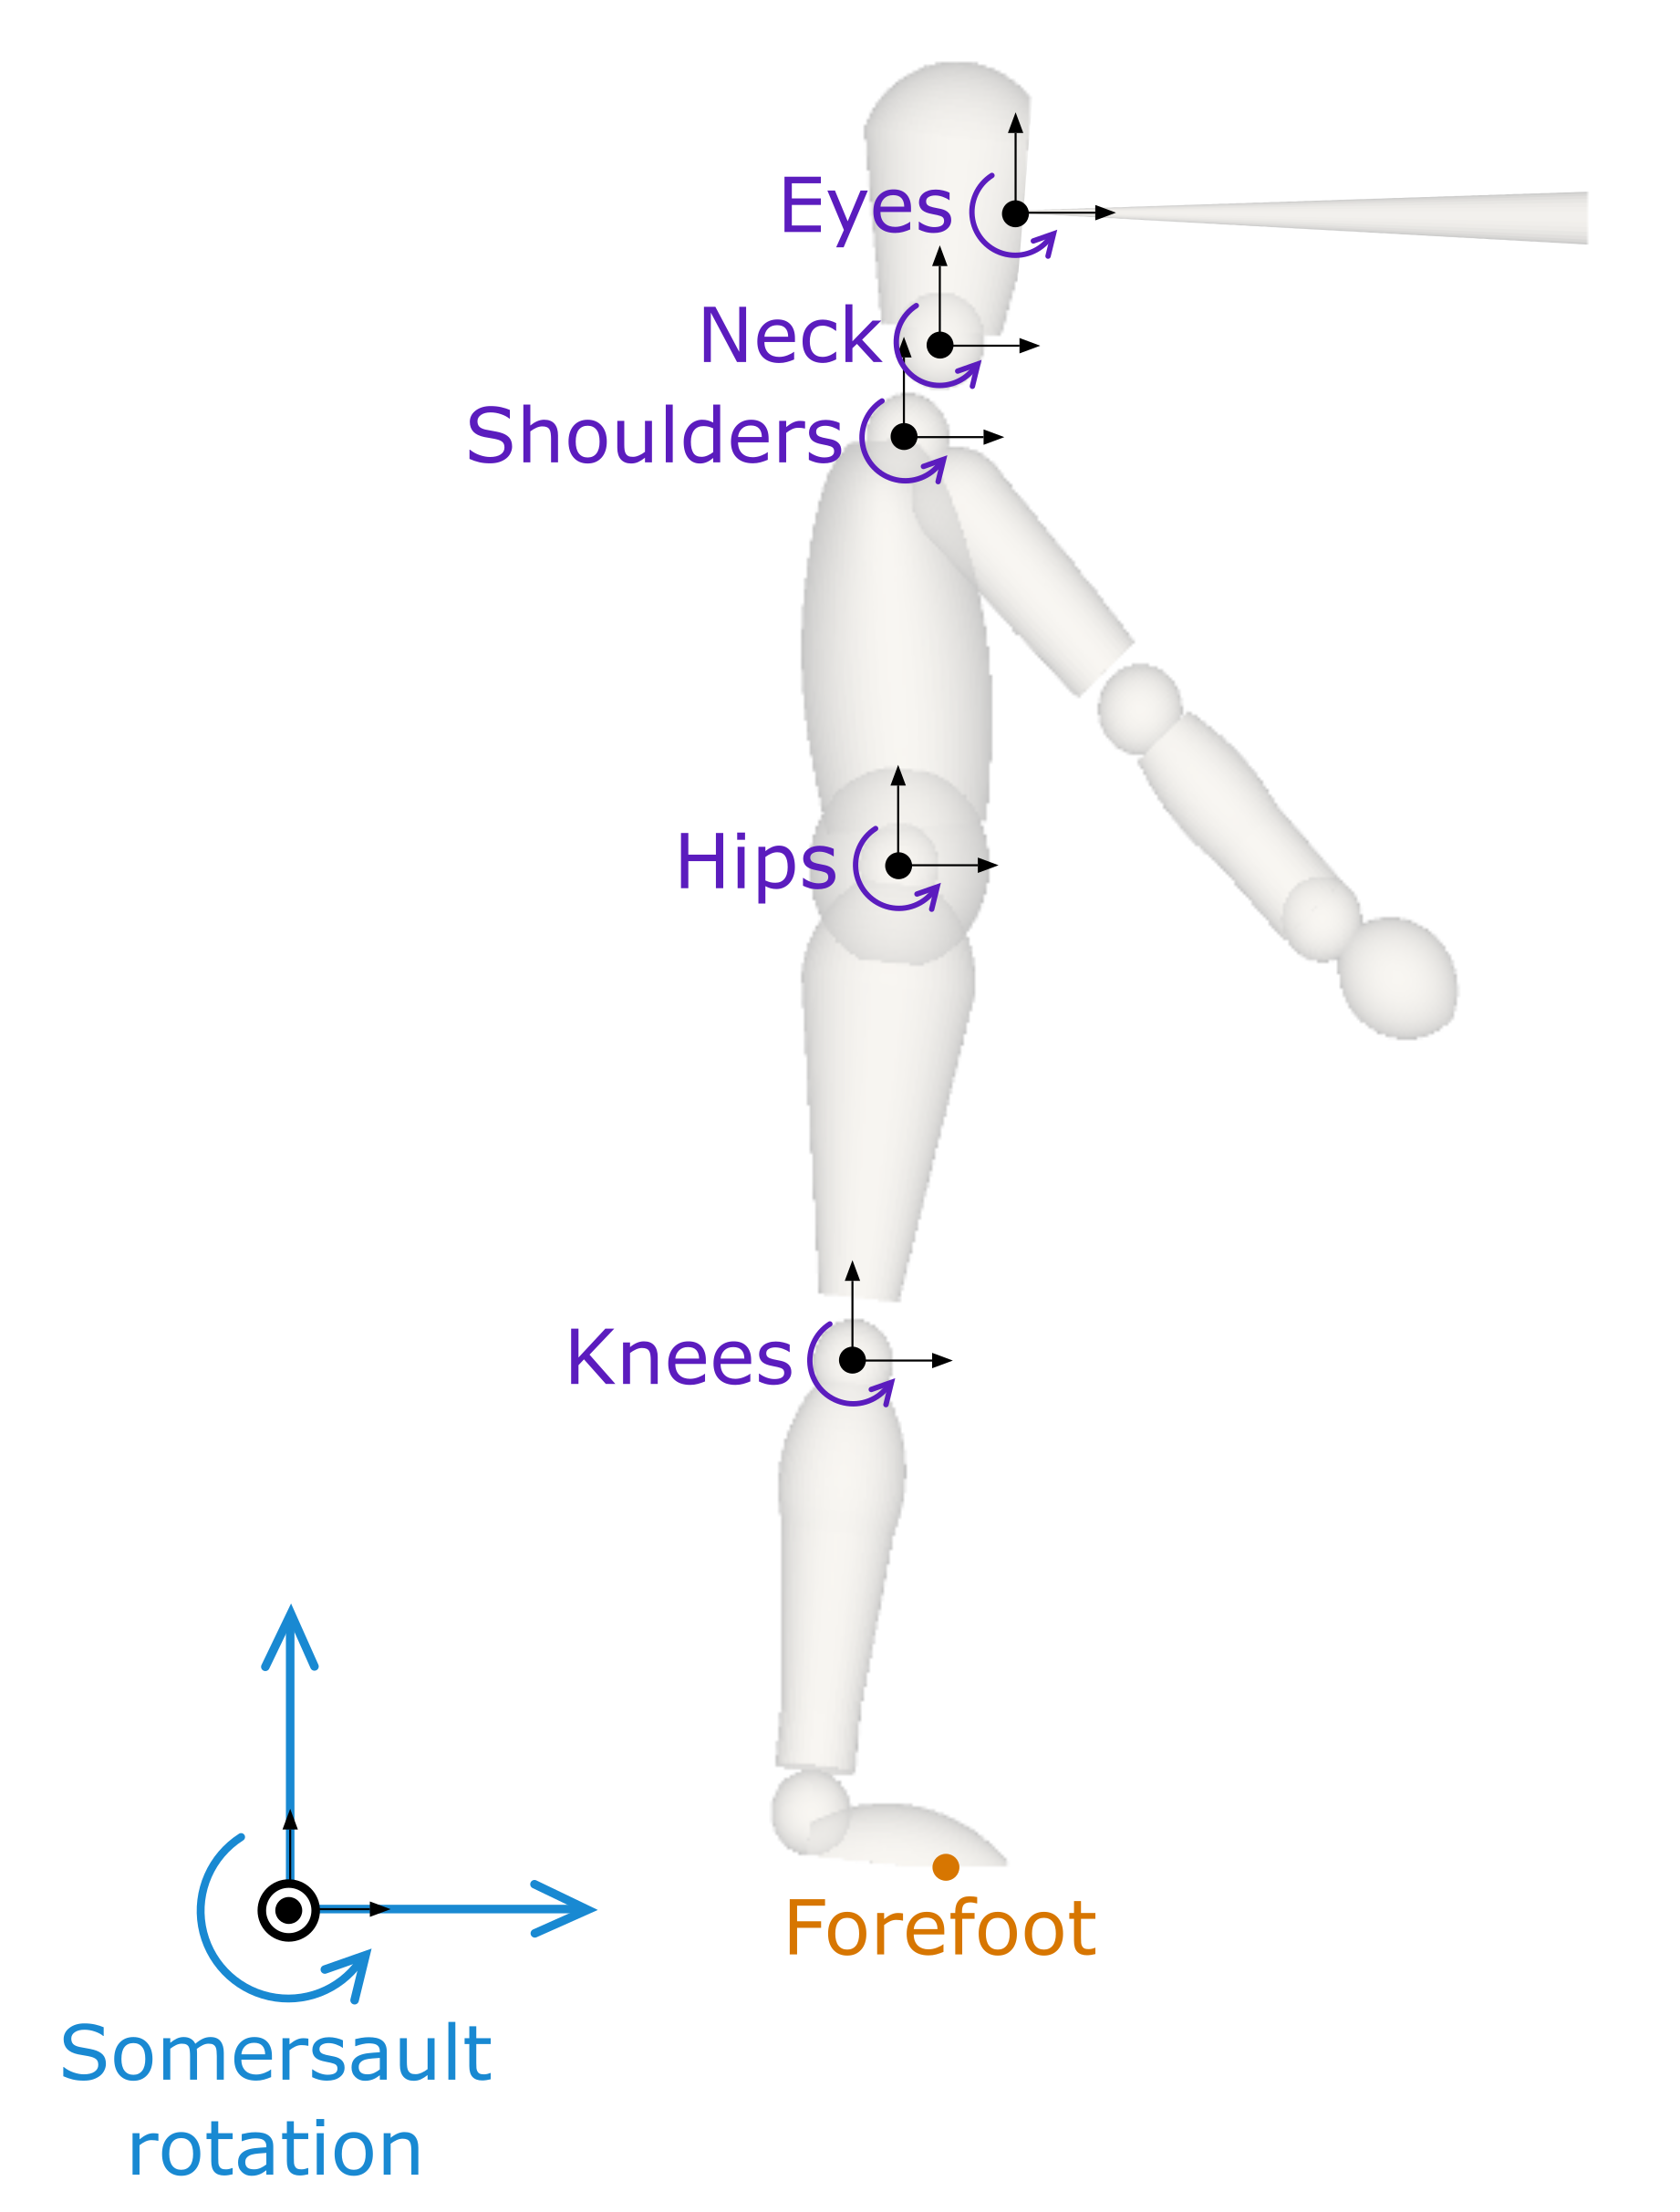
\includegraphics[width=0.5\linewidth]{figures/model.png}
\caption{The five-segment athletic avatar used for the predictive simulations. It is composed of three unactuated degrees of freedom (blue): forward translation, upward translation, and somersault rotation and five torque-actuated degrees of freedom (purple): neck, eye, shoulder, hip, and knee rotations. Note that the eye rotation was only used in the SOCP$^{\text{AF}}$ and SOCP$_{\text{VN}}^{\text{AF}}$ simulations (see Sec.~\ref{sec:methods_DSOCP} for more details).}
\label{fig:model}
\end{figure}

The athletic avatar's generalized coordinates ($q$) comprised unactuated (forward translation, upward translation, and somersault rotation) and torque-actuated degrees of freedom (DoFs).
All joints but the eyes (neck, shoulder, hip, and knee) were dampened by joint damping $- 0.1~\dot{q}$.
No torque was applied to each of the unactuated DoFs.
The torque applied on each actuated DoF ($\tau_{\text{total}}$) was composed of different components depending on the implementation considered (see Sec.~\ref{subsec:OCP}-\ref{subsec:SOCP_plus}).
The avatar was governed by the non-linear multibody dynamics equation:

\begin{equation}
F : 
	\begin{bmatrix}
	\ddot{q}^{\text{B}}  \\
	\ddot{q}^{\text{J}}
	\end{bmatrix}
	= M(q)^{-1} \left(
	{\begin{bmatrix}
	0_3 \\
	\tau_{\text{total}}
	\end{bmatrix}
	- N(q, \dot{q}) - 
	\begin{bmatrix}
	0 \\
	0 \\
	0 \\
	0.1 \\
	0 \\
	0.1 \\
	0.1 \\
	0.1
	\end{bmatrix}
	\dot{q}} \right) \label{eq:dynamics}
\end{equation}

\noindent where $q$, $\dot{q}$ and $\ddot{q}$ are the generalized joint coordinates, velocities and accelerations, respectively. $\ddot{q}^{\text{B}}$ refers to the joint acceleration of the unactuated (forward translation, upward translation, and somersault rotation) and $\ddot{q}^{\text{J}}$ to the actuated (neck, eye, shoulder, hip, and knee) DoFs. $\tau_{\text{total}}$ are the torques applied on each joint, $M$ is the mass matrix, $N$ is the non-linear effect vector comprising Coriolis, centrifugal, and gravity effects, and $v$ are the damping coefficient set to $0.1~sNm$ for the neck, shoulder, hip, and knee joints and to $0~sNm$ for the unactuated DoFs and the eyes.


\subsection{Discretized stochastic optimal control framework}\label{sec:methods_DSOCP}
% \comEC{In this section, remove some heavy math to put in appendices}
To transcribe the stochastic optimal control problems into a solvable deterministic optimal control problem, the motor and sensory noises were sampled from a Gaussian distribution at 20 different instances, as in \cite{koelewijn2020solution}.
Analogously, it could be viewed as 20 optimal control problems being solved simultaneously, each with different random motor and sensory noise values and thus different state values, but with the same motor command.
The number of noise samples (referred to as episodes) was chosen based on the analysis in \cite{koelewijn2020solution}.
They showed that the cost function value varied by less than 1\% when using 20 or more samples.
The constant part of the motor and sensory noises ($w_{\circ}$) were sampled from a Gaussian distribution with a standard deviation of $5$ for the joint torque motor noise, $0.0005$ for the joint angle proprioception, $0.0045$ for the joint velocity proprioception inputs, $0.0005$ for the vestibular input, and $0.0005$ for the visual inputs. 

The optimal policies were computed using a composite cost function, where the main objective was to minimize landing condition variability.
Other terms were added to the cost function to minimize the expected effort and its time derivative.
Finally, regularization terms were added to encourage a realistic motion: minimizing the movement duration, the direct feedback gains, and the rate of change of the direct feedback gains.
The optimization problems were implemented in Bioptim \cite{michaud2022bioptim} using the automatic differentiation provided by CasADi \cite{Andersson2019}, and solved using IPOPT \cite{wachter2006implementation} and the linear solver MA97 \cite{hogg2011hsl_ma97} with a tolerance of \num{1e-6}.
Each stochastic optimal control problem was warm-started with the optimal generalized coordinates, velocities and torques obtained from the deterministic solution.

To test our hypothesis, five different implementations of the problem were solved to generate optimal techniques for the aerial phase of a backward somersault (Tab.~\ref{tab:formulations}).

\begin{table}[h]
\centering
\caption{Features of the five optimal control implementations used, and the hypothesis they allow to verify.}\label{tab:formulations}
\begin{tabular}{lcccccc}
\toprule
 & \textbf{Stochastic} & \makecell{\textbf{Direct} \\ \textbf{feedback}} & \makecell{\textbf{Anticipatory} \\ \textbf{feedback}} & \makecell{\textbf{State-dependent} \\ \textbf{sensory noise}} & \makecell{\textbf{Control-dependent} \\ \textbf{motor noise}} &  \\
\midrule
\textcolor{OCP_color}{OCP} & & & & & &  \\
\textcolor{SOCP_color}{SOCP} & \checkmark & \checkmark & & & & \textbf{H1} \\
\textcolor{SOCP_FEEDFORWARD_color}{SOCP$^{\text{AF}}$} & \checkmark & \checkmark & \checkmark & & & \textbf{H2} \\
\textcolor{SOCP_VARIABLE_color}{SOCP$_{\text{VN}}$} & \checkmark & \checkmark & & \checkmark & \checkmark & \textbf{H3} \\
\textcolor{SOCP_plus_color}{SOCP$_{\text{VN}}^{\text{AF}}$} & \checkmark & \checkmark & \checkmark & \checkmark & \checkmark & \textbf{H4}  \\
\bottomrule
\end{tabular}
\end{table}


All implementations of optimal control problems are detailed in the following sections.
To simplify interpretation, each optimization variable is presented in colour.


\subsubsection{Deterministic optimal control problem (\textcolor{OCP_color}{OCP})}\label{subsec:OCP}
The deterministic implementation did not account for motor or sensory noise and consisted of a single episode (Fig.~\ref{fig:ocp}).
The torques applied to the joints were only composed of the voluntary motor command ($\textcolor{OCP_color}{\tau_{\text{voluntary}}}$).

% \begin{equation}
% \tau_{\text{total}} = \textcolor{OCP_color}{\tau_{\text{voluntary}}}
% \end{equation}

\begin{figure}[H]
\centering
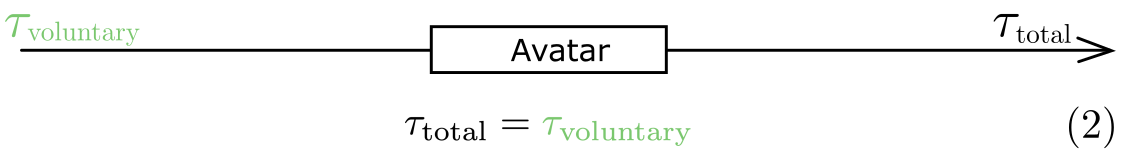
\includegraphics[width=1.0\linewidth]{figures/ocp.png}
\caption{A schematic and mathematical representation of the torques applied to the joints in the OCP implementation.}
\label{fig:ocp}
\end{figure}


\subsubsection{Stochastic optimal control problem (\textcolor{SOCP_color}{SOCP})}\label{subsec:SOCP}
The basic stochastic implementation was composed of 20 episodes (Fig.~\ref{fig:socp}). 
For each episode, motor and sensory noises were directly sampled from a Gaussian distribution.
The torques applied to the joints were composed of the voluntary motor command ($\textcolor{SOCP_color}{\tau_{\text{voluntary}}}$), direct feedback corrections ($\tau_{\text{dfb}}$), and motor noise ($\tau_{\text{noise}}$).
The direct feedback corrections were based on proprioceptive (joint positions and velocities) and vestibular (body spatial orientation) information. 
The direct feedback corrections applied to the joint torques ($\tau_{\text{dfb}}$ defined in Eq.~\figeq{fig:socp}{4}) were a linear combination (feedback gain matrix: $\textcolor{SOCP_color}{K_{\text{dfb}}}$) of the differences between the current noisy sensory information and a sensory reference ($\textcolor{SOCP_color}{\text{ref}_{\text{dfb}}}$).
The sensory reference was constrained to represent the mean sensory information across all episodes.
The sensory information was corrupted by random noise ($w_{\text{p}}$ and $w_{\text{v}}$).

% \begin{equation}
% \textcolor{SOCP_color}{K_{\text{dfb}}} \left({\text{ref}}_{\text{dfb}} 
% \begin{bmatrix}
% \textcolor{SOCP_color}{{q_n}^{\text{J}}} \\
% \textcolor{SOCP_color}{\mathop{\dot{q}_n}^{\text{J}}} \\
% \textcolor{SOCP_color}{{q_n}^{\text{S}}} \\
% \dot{\theta}_n \\
% \end{bmatrix} 
% + 
% \begin{bmatrix}
% w_p \\
% w_p \\
% w_v \\
% w_v \\
% \end{bmatrix} \right)
% \end{equation}

% \begin{equation}
% \tau_{\text{total}} = \textcolor{SOCP_color}{\tau_{\text{voluntary}}} + \tau_{\text{dfb}}(\textcolor{SOCP_color}{K_{\text{dfb}}}, \textcolor{SOCP_color}{q_n}, \textcolor{SOCP_color}{\dot{q}_n}, w_{\text{p}}, w_{\text{v}}) + \tau_{\text{noise}}(w_{\text{motor}})
% \end{equation}

% \begin{equation}
% \tau_{\text{dfb}} = \textcolor{SOCP_color}{K_{\text{dfb}}} (\textcolor{SOCP_color}{\text{ref}_{\text{dfb}}} - S_{\text{dfb}}^{\text{SOCP}}(\textcolor{SOCP_color}{q_n}, \textcolor{SOCP_color}{\dot{q}_n}, w_{\text{p}}, w_{\text{v}}))
% \end{equation}
% \begin{equation}
% S_{\text{dfb}}^{\text{SOCP}} = 
% \begin{bmatrix}
% \textcolor{SOCP_color}{{q_n}^{\text{J}}} \\
% \textcolor{SOCP_color}{\mathop{\dot{q}_n}^{\text{J}}} \\
% \textcolor{SOCP_color}{{q_n}^{\text{S}}} \\
% \dot{\theta}_n(\textcolor{SOCP_color}{q_n}, \textcolor{SOCP_color}{\dot{q}_n})
% \end{bmatrix} + 
% \begin{bmatrix}
% w_{\text{p}} \\
% w_{\text{p}} \\
% w_{\text{v}} \\
% w_{\text{v}}
% \end{bmatrix}
% \end{equation}
% \begin{equation}
% \tau_{\text{noise}} = w_{\text{motor}}
% \end{equation}

\begin{figure}[H]
\centering
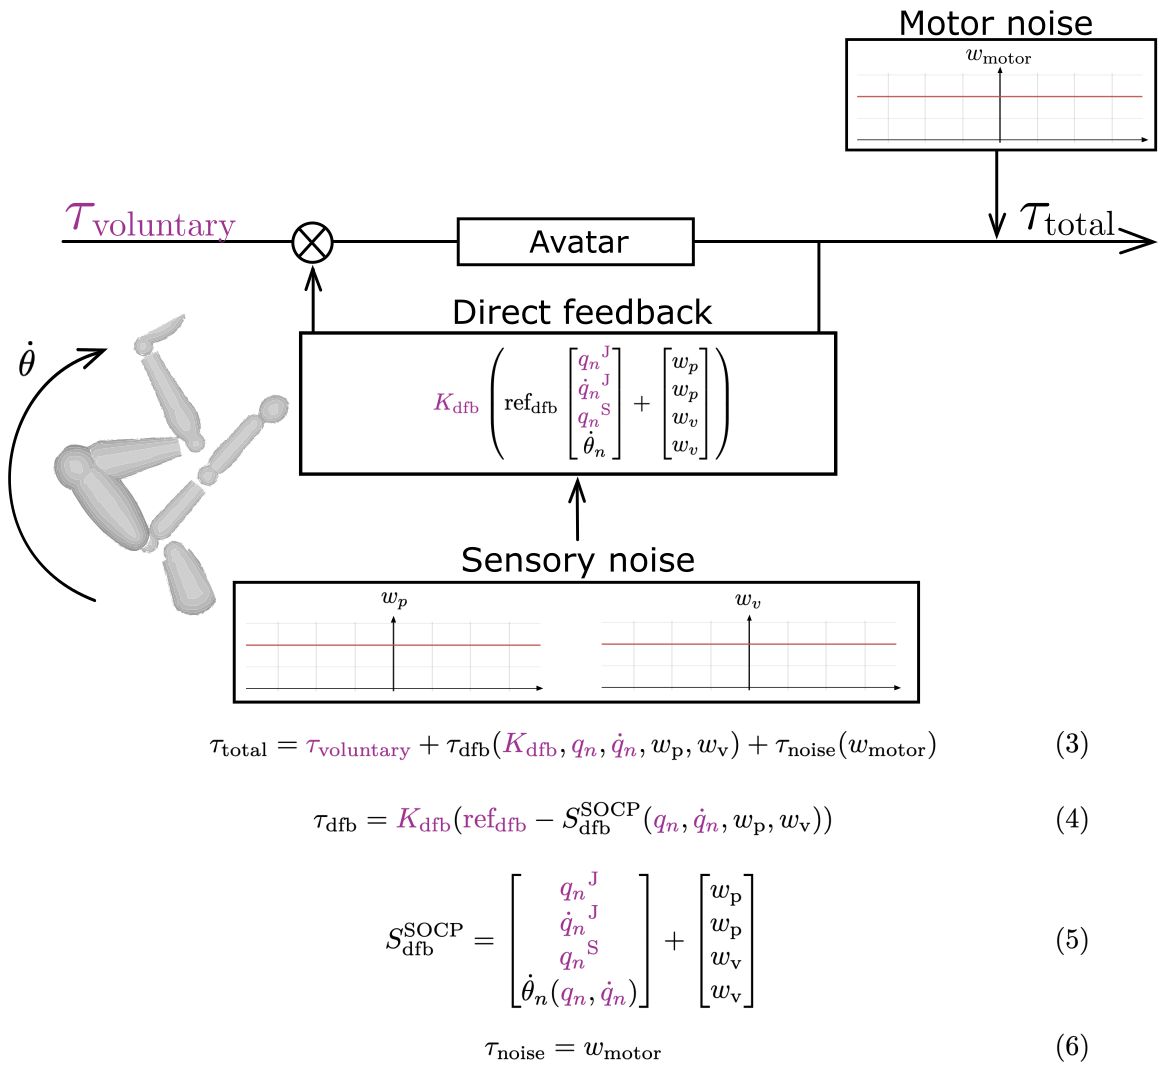
\includegraphics[width=1.0\linewidth]{figures/socp.png}
\caption{A schematic and mathematical representation of the torques applied to the joints in the SOCP implementation. The $._n$ indices relate to the $n^{th}$ episode.}
\label{fig:socp}
\end{figure}


\subsubsection{Stochastic optimal control problem with variable noises (\textcolor{SOCP_VARIABLE_color}{SOCP$_{\text{VN}}$})}\label{subsec:SOCPV}
The first improved stochastic implementation considered signal-dependent motor noise and state-dependent sensory noise (Fig.~\ref{fig:socp_variable}).
The torques applied to the joints were composed of the voluntary motor command ($\textcolor{SOCP_VARIABLE_color}{\tau_{\text{voluntary}}}$), direct feedback corrections ($\tau_{\text{dfb}}$), and motor noise ($\tau_{\text{noise}}$).
The direct feedback corrections were identical to those in the SOCP implementation.
However, the vestibular information was corrupted by state-dependent random noise ($c_s$) through an inverted Gaussian function, such that the reliability of the vestibular information increased as the head angular velocity in the global reference frame ($H$) decreased.
The motor command was corrupted by signal-dependent random noise ($c_{motor}$) through an inverted Gaussian function, such that the accuracy of the joint torques decreased as the voluntary motor command increased.

% \begin{equation}
% \textcolor{SOCP_VARIABLE_color}{K_{\text{dfb}}} \left({\text{ref}}_{\text{dfb}} 
% \begin{bmatrix}
% \textcolor{SOCP_VARIABLE_color}{{q_n}^{\text{J}}} \\
% \textcolor{SOCP_VARIABLE_color}{\mathop{\dot{q}_n}^{\text{J}}} \\
% \textcolor{SOCP_VARIABLE_color}{{q_n}^{\text{S}}} \\
% \dot{\theta}_n \\
% \end{bmatrix} 
% + 
% \begin{bmatrix}
% w_p \\
% w_p \\
% C_v \\
% C_v \\
% \end{bmatrix} \right)
% \end{equation}

% \begin{equation}
% H
% \end{equation}

% \begin{equation}
% \tau_{\text{total}} = \textcolor{SOCP_VARIABLE_color}{\tau_{\text{voluntary}}} + \tau_{\text{dfb}}(\textcolor{SOCP_VARIABLE_color}{K_{\text{dfb}}}, \textcolor{SOCP_VARIABLE_color}{q_n}, \textcolor{SOCP_VARIABLE_color}{\dot{q}_n}, w_{\text{p}}, w_{\text{v}}) + \tau_{\text{noise}}(\textcolor{SOCP_VARIABLE_color}{\tau_{\text{voluntary}}}, w_{\text{motor}})
% \end{equation}

% \begin{equation}
% \tau_{\text{dfb}} = \textcolor{SOCP_VARIABLE_color}{K_{\text{dfb}}} (\textcolor{SOCP_VARIABLE_color}{\text{ref}_{\text{dfb}}} - S_{\text{dfb}}^{\text{SOCP}_{\text{VN}}}(\textcolor{SOCP_VARIABLE_color}{q_n}, \textcolor{SOCP_VARIABLE_color}{\dot{q}_n}, w_{\text{p}}, w_{\text{v}}))
% \end{equation}
% \begin{equation}
% S_{\text{dfb}}^{\text{SOCP}_{\text{VN}}} =
% \begin{bmatrix}
% \textcolor{SOCP_VARIABLE_color}{{q_n}^{\text{J}}} \\
% \textcolor{SOCP_VARIABLE_color}{\mathop{\dot{q}_n}^{\text{J}}} \\
% \textcolor{SOCP_VARIABLE_color}{{q_n}^{\text{S}}} \\
% \dot{\theta}_n(\textcolor{SOCP_VARIABLE_color}{q_n}, \textcolor{SOCP_VARIABLE_color}{\dot{q}_n})
% \end{bmatrix} +
% \begin{bmatrix}
% w_{\text{p}} \\
% w_{\text{p}} \\
% \frac{-1}{\sqrt{2 \pi}} e^{(-0.5 (\frac{H(\textcolor{SOCP_VARIABLE_color}{q_n}, \textcolor{SOCP_VARIABLE_color}{\dot{q}_n})}{10})^2)}
% + \frac{w_{\text{v}}}{\sqrt{2 \pi}} \\
% \frac{-1}{\sqrt{2 \pi}} e^{(-0.5 (\frac{H(\textcolor{SOCP_VARIABLE_color}{q_n}, \textcolor{SOCP_VARIABLE_color}{\dot{q}_n})}{10})^2)}
% + \frac{w_{\text{v}}}{\sqrt{2 \pi}}
% \end{bmatrix}
% \end{equation}
% \begin{equation}
% \tau_{\text{noise}} = \frac{-10}{\sqrt{2 \pi}} e^{(-0.5 (\frac{\textcolor{SOCP_VARIABLE_color}{\tau_{\text{voluntary}}}}{1000})^2)} + w_{\text{motor}} + \frac{10~w_{\text{motor}}}{\sqrt{2 \pi}}
% \end{equation}

\begin{figure}[H]
\centering
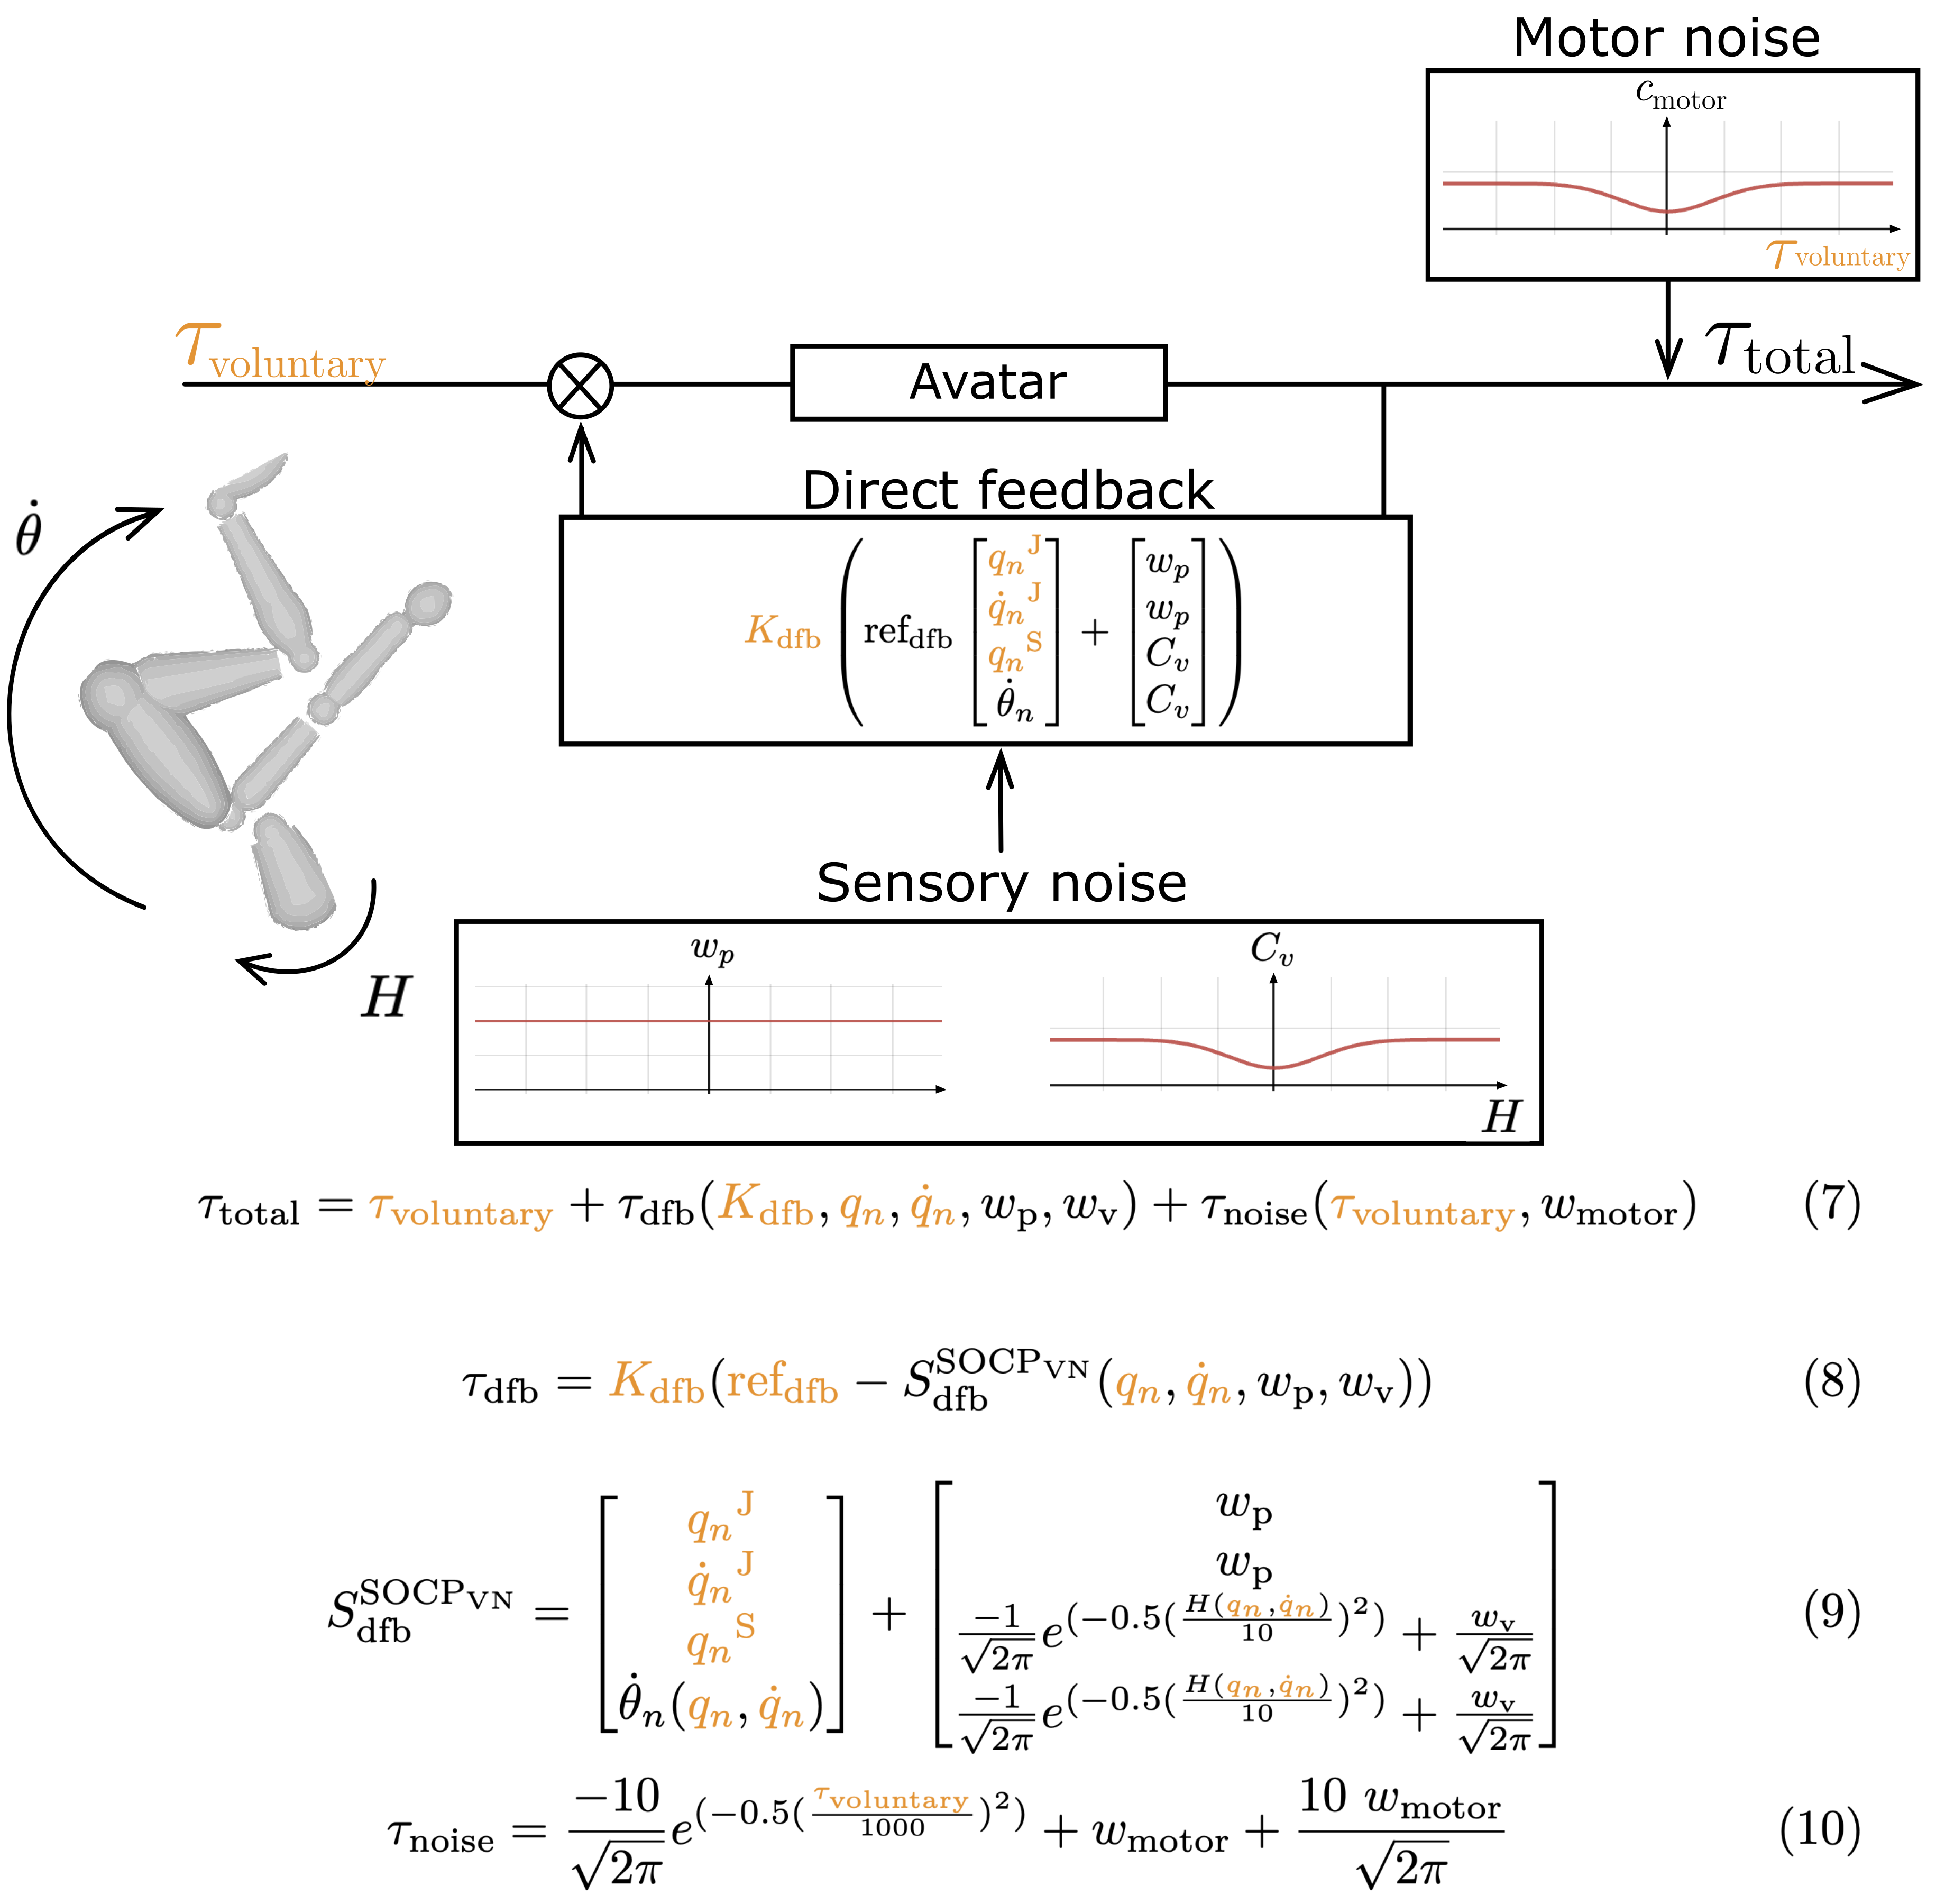
\includegraphics[width=1.0\linewidth]{figures/socp_variable.png}
\caption{A schematic and mathematical representation of the torques applied to the joints in the SOCP$_{\text{VN}}$ implementation.}
\label{fig:socp_variable}
\end{figure}


\subsubsection{Stochastic optimal control problem with anticipatory feedback (\textcolor{SOCP_FEEDFORWARD_color}{SOCP$^{\text{AF}}$})}\label{subsec:SOCPA}
The second improved stochastic implementation accounted for random motor and sensory noise by directly sampling from a Gaussian distribution (Fig.~\ref{fig:socp_feedforward}).
The torques applied to the joints were composed of the voluntary motor command ($\textcolor{SOCP_FEEDFORWARD_color}{\tau_{\text{voluntary}}}$), direct feedback corrections ($\tau_{\text{dfb}}$), anticipatory feedback corrections ($\tau_{\text{afb}}$), and motor noise ($\tau_{\text{noise}}$).
The direct feedback corrections were identical to those in the SOCP implementation.
The anticipatory feedback corrections were based on visual (time remaining until landing: $\textcolor{SOCP_FEEDFORWARD_color}{T} - t_i$) and vestibular (body spatial orientation: $\textcolor{SOCP_FEEDFORWARD_color}{{q_n}_\text{S}}$ and somersault velocity: $\dot{\theta}$) information. 
An Euler integration was used as a forward model to estimate the body orientation at landing from the sensory information.
The anticipatory feedback corrections applied to the joint torques ($\tau_{\text{afb}}$) were proportional (feedback gain vector: $\textcolor{SOCP_FEEDFORWARD_color}{K_{\text{afb}}}$) to the difference between the current noisy sensory information and a sensory reference ($2\pi$: a full somersault rotation at landing).
The sensory information was corrupted by random noise ($w_{\text{v/g}}$).

% \begin{equation}
% \textcolor{SOCP_FEEDFORWARD_color}{K_{\text{dfb}}} \left({\text{ref}}_{\text{dfb}} 
% \begin{bmatrix}
% \textcolor{SOCP_FEEDFORWARD_color}{{q_n}^{\text{J}}} \\
% \textcolor{SOCP_FEEDFORWARD_color}{\mathop{\dot{q}_n}^{\text{J}}} \\
% \textcolor{SOCP_FEEDFORWARD_color}{{q_n}^{\text{S}}} \\
% \dot{\theta}_n \\
% \end{bmatrix} 
% + 
% \begin{bmatrix}
% w_p \\
% w_p \\
% w_v \\
% w_v \\
% \end{bmatrix} \right)
% \end{equation}

% \begin{equation}
% \textcolor{SOCP_FEEDFORWARD_color}{K_{\text{afb}}} \left(2\pi - (\textcolor{SOCP_FEEDFORWARD_color}{{q_n}^{\text{S}}} + \dot{\theta}_n (\textcolor{SOCP_FEEDFORWARD_color}{T} - t_i)) + w_v \right)
% \end{equation}

% \begin{eqnarray}
% \tau_{\text{total}} = \textcolor{SOCP_FEEDFORWARD_color}{\tau_{\text{voluntary}}} + \tau_{\text{dfb}}(\textcolor{SOCP_FEEDFORWARD_color}{K_{\text{dfb}}}, \textcolor{SOCP_FEEDFORWARD_color}{q_n}, \textcolor{SOCP_FEEDFORWARD_color}{\dot{q}_n}, w_{\text{p}}, w_{\text{v}}) + \nonumber\\
% \tau_{\text{afb}}(\textcolor{SOCP_FEEDFORWARD_color}{K_{\text{afb}}}, \textcolor{SOCP_FEEDFORWARD_color}{q_n}, \textcolor{SOCP_FEEDFORWARD_color}{\dot{q}_n}, w_{\text{v/g}}) + \tau_{\text{noise}}(w_{\text{motor}})
% \end{eqnarray}

% \begin{equation}
% \tau_{\text{dfb}} = \textcolor{SOCP_FEEDFORWARD_color}{K_{\text{dfb}}} (\textcolor{SOCP_FEEDFORWARD_color}{\text{ref}_{\text{dfb}}} - S_{\text{dfb}}^{\text{SOCP}^{\text{AF}}}(\textcolor{SOCP_FEEDFORWARD_color}{q_n}, \textcolor{SOCP_FEEDFORWARD_color}{\dot{q}_n}, w_{\text{p}}, w_{\text{v}}))
% \end{equation}
% \begin{equation}
% S_{\text{dfb}}^{\text{SOCP}^{\text{AF}}} = 
% \begin{bmatrix}
% \textcolor{SOCP_FEEDFORWARD_color}{{q_n}^{\text{J}}} \\
% \textcolor{SOCP_FEEDFORWARD_color}{\mathop{\dot{q}_n}^{\text{J}}} \\
% \textcolor{SOCP_FEEDFORWARD_color}{{q_n}^{\text{S}}}
% \end{bmatrix} + 
% \begin{bmatrix}
% w_{\text{p}} \\
% w_{\text{p}} \\
% w_{\text{v}}
% \end{bmatrix}
% \end{equation}
% \begin{equation}
% \tau_{\text{afb}} = \textcolor{SOCP_FEEDFORWARD_color}{K_{\text{afb}}} (\text{ref}_{\text{afb}} - S_{\text{afb}}^{\text{SOCP}^{\text{AF}}}(\textcolor{SOCP_FEEDFORWARD_color}{q_n}, \textcolor{SOCP_FEEDFORWARD_color}{\dot{q}_n}, w_{\text{p}}, w_{\text{v/g}})
% \end{equation}
% \begin{equation}
% S_{\text{afb}}^{\text{SOCP}^{\text{AF}}} = \textcolor{SOCP_FEEDFORWARD_color}{{q_n}_{\text{S}}} + \dot{\theta}(\textcolor{SOCP_FEEDFORWARD_color}{q_n}, \textcolor{SOCP_FEEDFORWARD_color}{\dot{q}_n}) \centerdot T_{\text{remaining}}(\textcolor{SOCP_FEEDFORWARD_color}{T}) + w_{\text{v/g}}
% \end{equation}
% \begin{equation}
% \tilde{T}_{\text{remaining}} = \textcolor{SOCP_FEEDFORWARD_color}{T} - t_i
% \end{equation}
% \begin{equation}
% \text{ref}_{\text{afb}} = 2\pi
% \end{equation}
% \begin{equation}
% \tau_{\text{noise}} = w_{\text{motor}}
% \end{equation}

\begin{figure}[H]
\centering
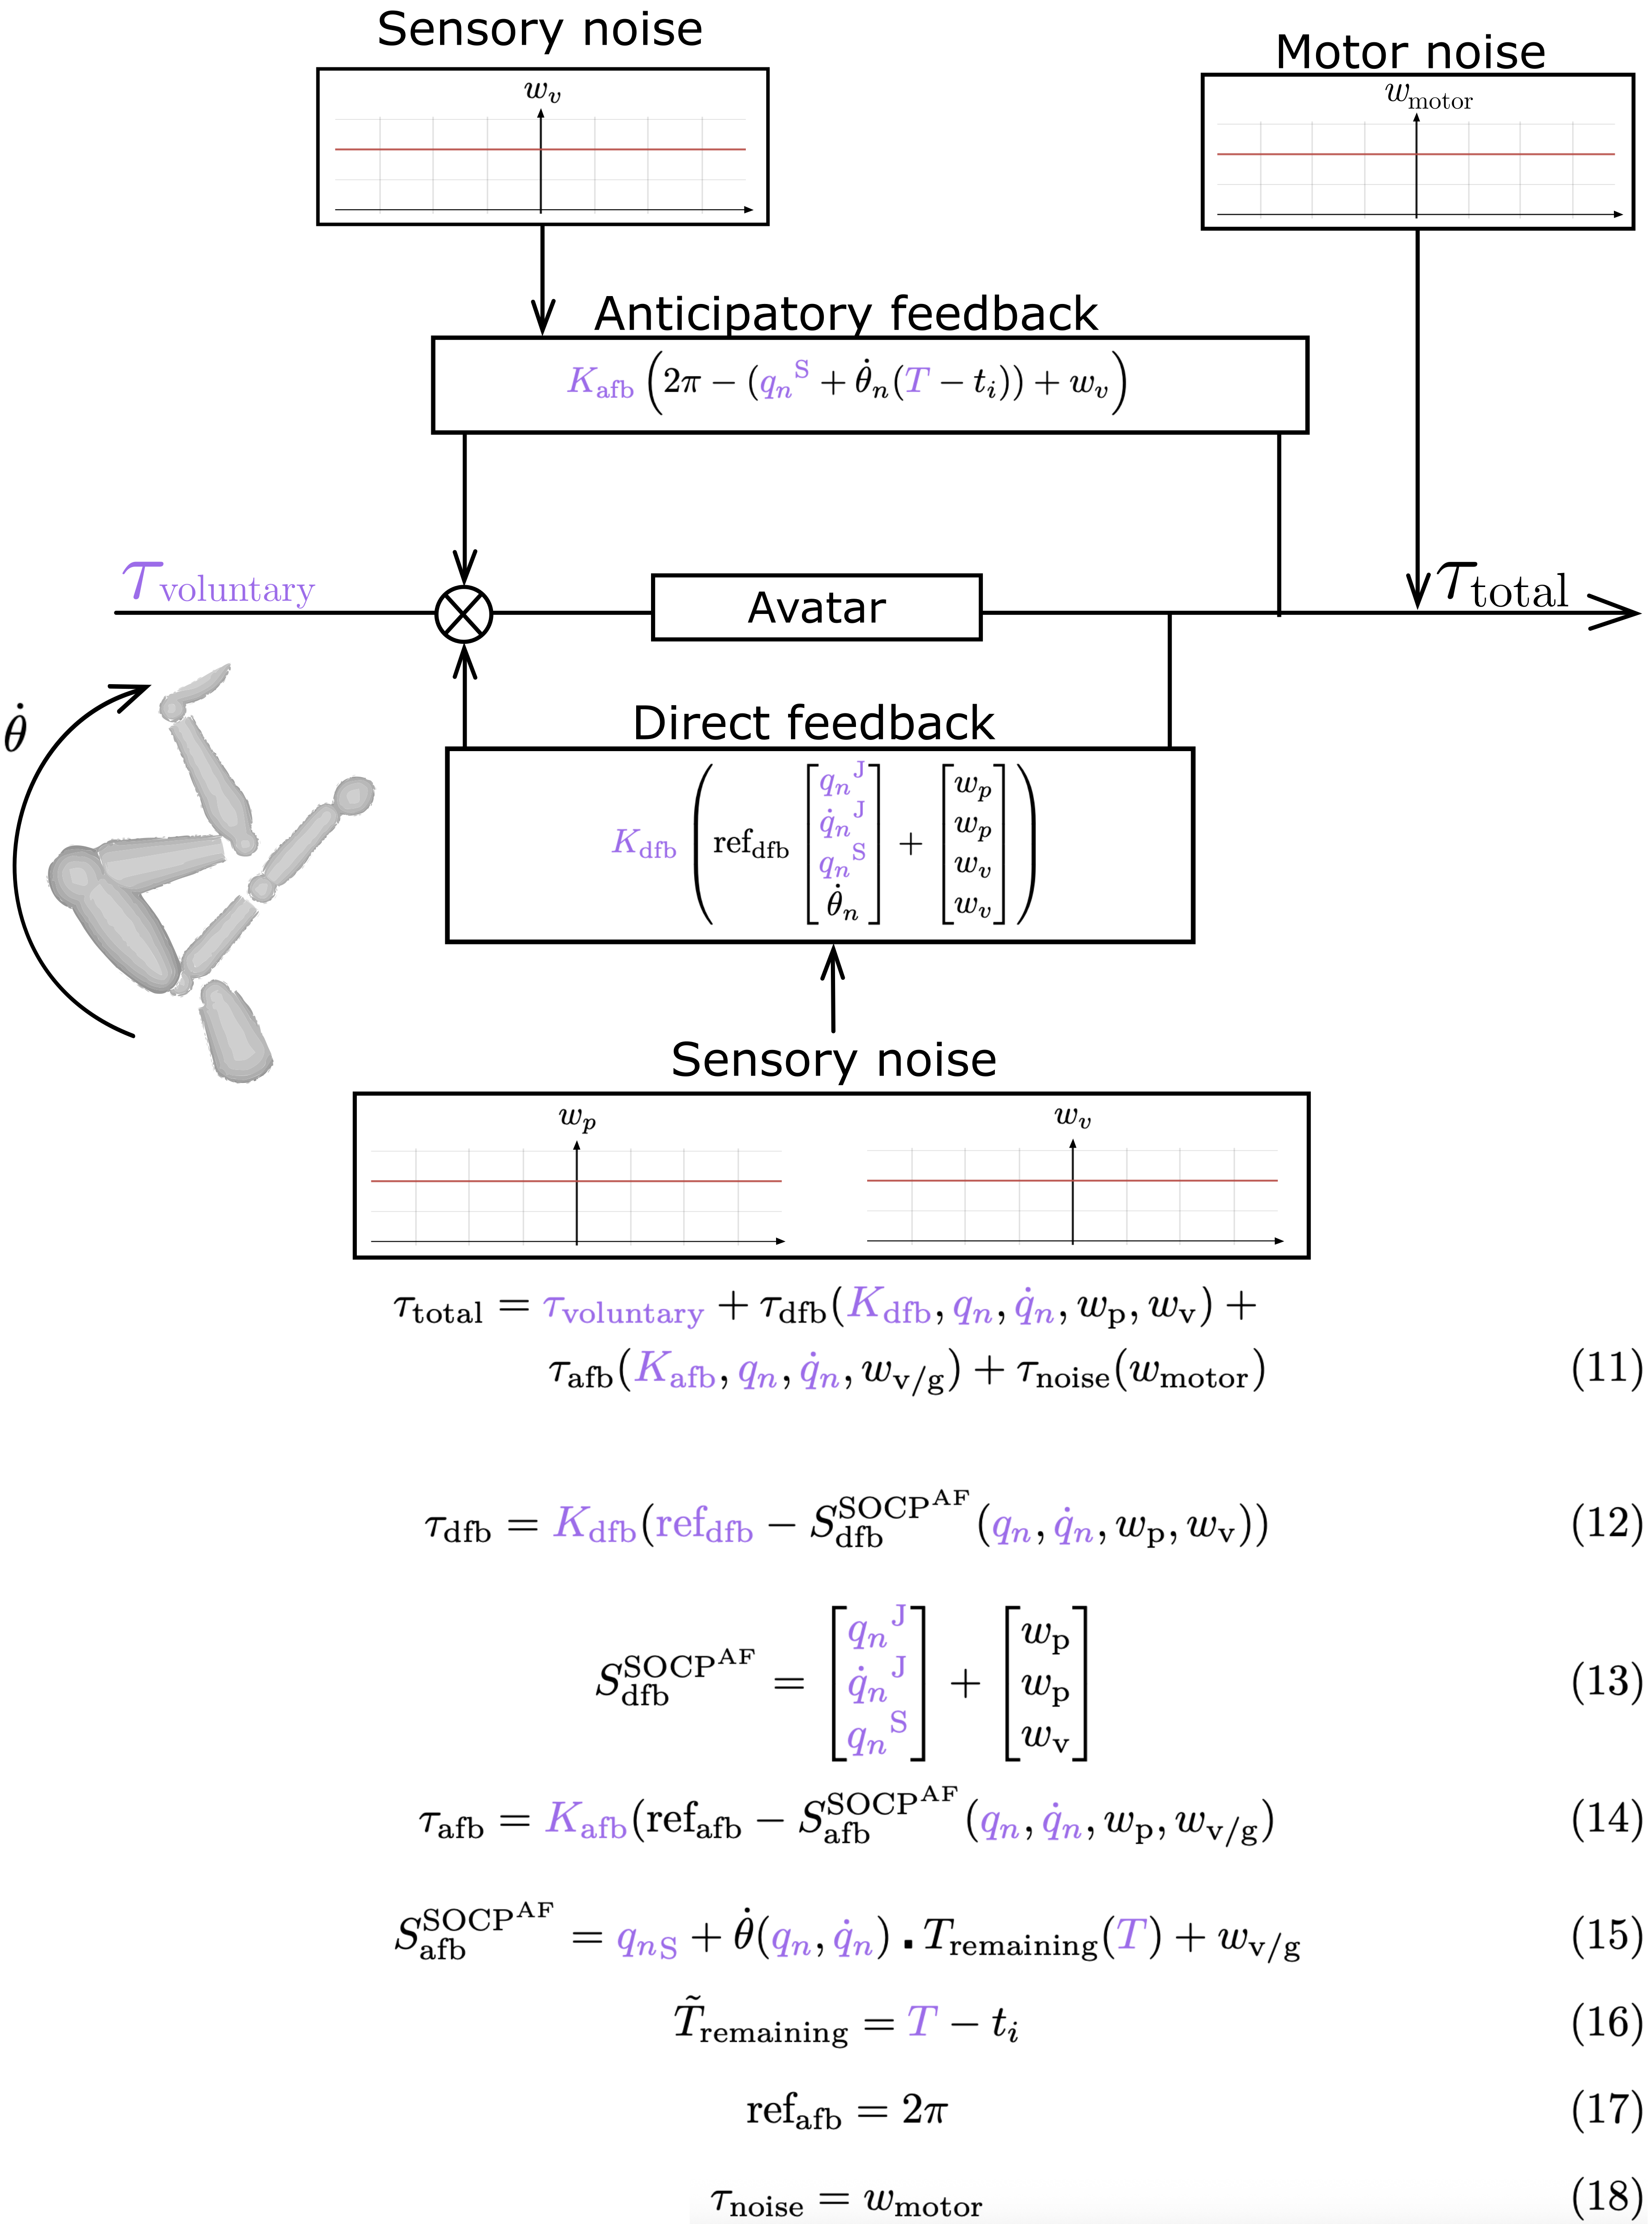
\includegraphics[width=1.0\linewidth]{figures/socp_feedforward.png}
\caption{A schematic and mathematical representation of the torques applied to the joints in the SOCP$^{\text{AF}}$ implementation. The index ${.}_i$ relates to the $i^{th}$ shooting node.}
\label{fig:socp_feedforward}
\end{figure}


\subsubsection{Stochastic optimal control problem with anticipatory feedback and variable noises (\textcolor{SOCP_plus_color}{SOCP$_{\text{VN}}^{\text{AF}}$})}\label{subsec:SOCP_plus}
This advanced stochastic implementation considered signal-dependent motor noise and state-dependent sensory noise (Fig.~\ref{fig:socp_plus}).
The torques applied to the joints were composed of the voluntary motor command ($\textcolor{SOCP_plus_color}{\tau_{\text{voluntary}}}$), direct feedback corrections ($\tau_{\text{dfb}}$), anticipatory feedback corrections ($\tau_{\text{afb}}$), and motor noise ($\tau_{\text{noise}}$).
The direct feedback corrections were identical to those of the SOCP implementation, and the anticipatory feedback corrections were identical to those of the SOCP$^{\text{AF}}$ implementation.
However, the vestibular information was corrupted by state-dependent random noise (${c_s}_{\text{v}}$) through an inverted Gaussian function, such that the corruption of the rotation rate information increased as the head angular velocity in the global reference frame ($H$) increased.
And the visual information was corrupted by state-dependent random noise (${c_s}_{\text{g}}$) through a smoothed square function, such that the corruption of the remaining time until landing information largely increased when the landing area was not visible (large $\measuredangle_{\text{gaze}}^{\text{floor}}$).
The motor command was corrupted by signal-dependent random noise ($c_{motor}$) through an inverted Gaussian function, such that the precision of the joint torques decreased as the voluntary motor command increased.

% \begin{equation}
% \textcolor{SOCP_plus_color}{K_{\text{dfb}}} \left({\text{ref}}_{\text{dfb}} 
% \begin{bmatrix}
% \textcolor{SOCP_plus_color}{{q_n}^{\text{J}}} \\
% \textcolor{SOCP_plus_color}{\mathop{\dot{q}_n}^{\text{J}}} \\
% \textcolor{SOCP_plus_color}{{q_n}^{\text{S}}} \\
% \dot{\theta}_n \\
% \end{bmatrix} 
% + 
% \begin{bmatrix}
% w_p \\
% w_p \\
% C_v \\
% C_v \\
% \end{bmatrix} \right)
% \end{equation}

% \begin{equation}
% \textcolor{SOCP_plus_color}{K_{\text{afb}}} \left(2\pi - ((\textcolor{SOCP_plus_color}{{q_n}^{\text{S}}} + C_v) + (\dot{\theta}_n (\textcolor{SOCP_plus_color}{T} - t_i) + C_g)) \right)
% \end{equation}

% \begin{eqnarray}
% \tau_{\text{total}} = \textcolor{SOCP_plus_color}{\tau_{\text{voluntary}}} + \tau_{\text{dfb}}(\textcolor{SOCP_plus_color}{K_{\text{dfb}}}, \textcolor{SOCP_plus_color}{q_n}, \textcolor{SOCP_plus_color}{\dot{q}_n}, w_{\text{p}}, w_{\text{v}}) + \nonumber \\
% \tau_{\text{afb}}(\textcolor{SOCP_plus_color}{K_{\text{afb}}}, \textcolor{SOCP_plus_color}{q_n}, \textcolor{SOCP_plus_color}{\dot{q}_n}, w_{\text{v/g}}) + \tau_{\text{noise}}(\textcolor{SOCP_plus_color}{\tau_{\text{voluntary}}}, w_{\text{motor}})
% \end{eqnarray}

% \begin{equation}
% \tau_{\text{dfb}} = \textcolor{SOCP_plus_color}{K_{\text{dfb}}} (\textcolor{SOCP_plus_color}{\text{ref}_{\text{dfb}}} - S_{\text{dfb}}^{\text{SOCP}_{\text{VN}}^{\text{AF}}}(\textcolor{SOCP_plus_color}{q_n}, \textcolor{SOCP_plus_color}{\dot{q}_n}, w_{\text{p}}, w_{\text{v}}))
% \end{equation}
% \begin{equation}
% S_{\text{dfb}}^{\text{SOCP}_{\text{VN}}^{\text{AF}}} =
% \begin{bmatrix}
% \textcolor{SOCP_plus_color}{{q_n}^{\text{J}}} \\
% \textcolor{SOCP_plus_color}{\mathop{\dot{q}_n}^{\text{J}}} \\
% \textcolor{SOCP_plus_color}{{q_n}^{\text{S}}}
% \end{bmatrix} +
% \begin{bmatrix}
% w_{\text{p}} \\
% w_{\text{p}} \\
% \frac{-1}{\sqrt{2 \pi}} e^{(-0.5 (\frac{H(\textcolor{SOCP_plus_color}{q_n}, \textcolor{SOCP_plus_color}{\dot{q}_n})}{10})^2)}
% + \frac{w_{\text{v}}}{\sqrt{2 \pi}}
% \end{bmatrix}
% \end{equation}
% \begin{equation}
% \tau_{\text{afb}} = \textcolor{SOCP_plus_color}{K_{\text{afb}}} (\text{ref}_{\text{afb}} - S_{\text{afb}}^{\text{SOCP}_{\text{VN}}^{\text{AF}}}(\textcolor{SOCP_plus_color}{q_n}, \textcolor{SOCP_plus_color}{\dot{q}_n}, w_{\text{p}}, w_{\text{v}}, w_{\text{g}})
% \end{equation}
% \begin{equation}
% S_{\text{afb}}^{\text{SOCP}_{\text{VN}}^{\text{AF}}} = {\tilde{q_n}}_{\text{S}}(\textcolor{SOCP_plus_color}{\dot{q}_n}, w_{\text{v}}) + \tilde{\dot{\theta}}(\textcolor{SOCP_plus_color}{q_n}, \textcolor{SOCP_plus_color}{\dot{q}_n}, w_{\text{v}}) \centerdot \tilde{T}_{\text{remaining}}(\textcolor{SOCP_plus_color}{T}, w_{\text{g}})
% \end{equation}
% \begin{equation}
% {\tilde{q_n}}_{\text{S}} = \textcolor{SOCP_plus_color}{{q_n}_{\text{S}}} + (\frac{-1}{\sqrt{2\pi}} e^{(-0.5 (\frac{H(\textcolor{SOCP_plus_color}{q_n}, \textcolor{SOCP_plus_color}{ \dot{q}_n})}{10})^2)} + \frac{w_{\text{v}}}{\sqrt{2\pi}})
% \end{equation}
% \begin{equation}
% \tilde{\dot{\theta}} = \dot{\theta}(\textcolor{SOCP_plus_color}{q_n}, \textcolor{SOCP_plus_color}{\dot{q}_n}) + (\frac{-1}{\sqrt{2 \pi}} e^{(-0.5 (\frac{H(\textcolor{SOCP_plus_color}{q_n}, \textcolor{SOCP_plus_color}{\dot{q}_n})}{10})^2)}
% + \frac{w_{\text{v}}}{\sqrt{2 \pi}})
% \end{equation}
% \begin{equation}
% \tilde{T}_{\text{remaining}} = \textcolor{SOCP_plus_color}{T} - \frac{\textcolor{SOCP_plus_color}{T}}{N} i + \frac{5~w_{\text{g}}~\sin{(0.5 \measuredangle_{\text{gaze}}^{\text{floor}} - \pi / 2)}}{\sqrt{0.1^2 + \sin{(0.5 \measuredangle_{\text{gaze}}^{\text{floor}} - \pi / 2)}^2}} + w_{\text{g}} + \frac{5~w_{\text{g}}}{\sqrt{0.1^2 + 1}}
% \end{equation}
% \begin{equation}
% \text{ref}_{\text{afb}} = 2\pi
% \end{equation}
% \begin{equation}
% \tau_{\text{noise}} = \frac{-10}{\sqrt{2 \pi}} e^{(-0.5 (\frac{\textcolor{SOCP_plus_color}{\tau_{\text{voluntary}}}}{1000})^2)} + w_{\text{motor}} + \frac{10~w_{\text{motor}}}{\sqrt{2 \pi}}
% \end{equation}

\begin{figure}[H]
\centering
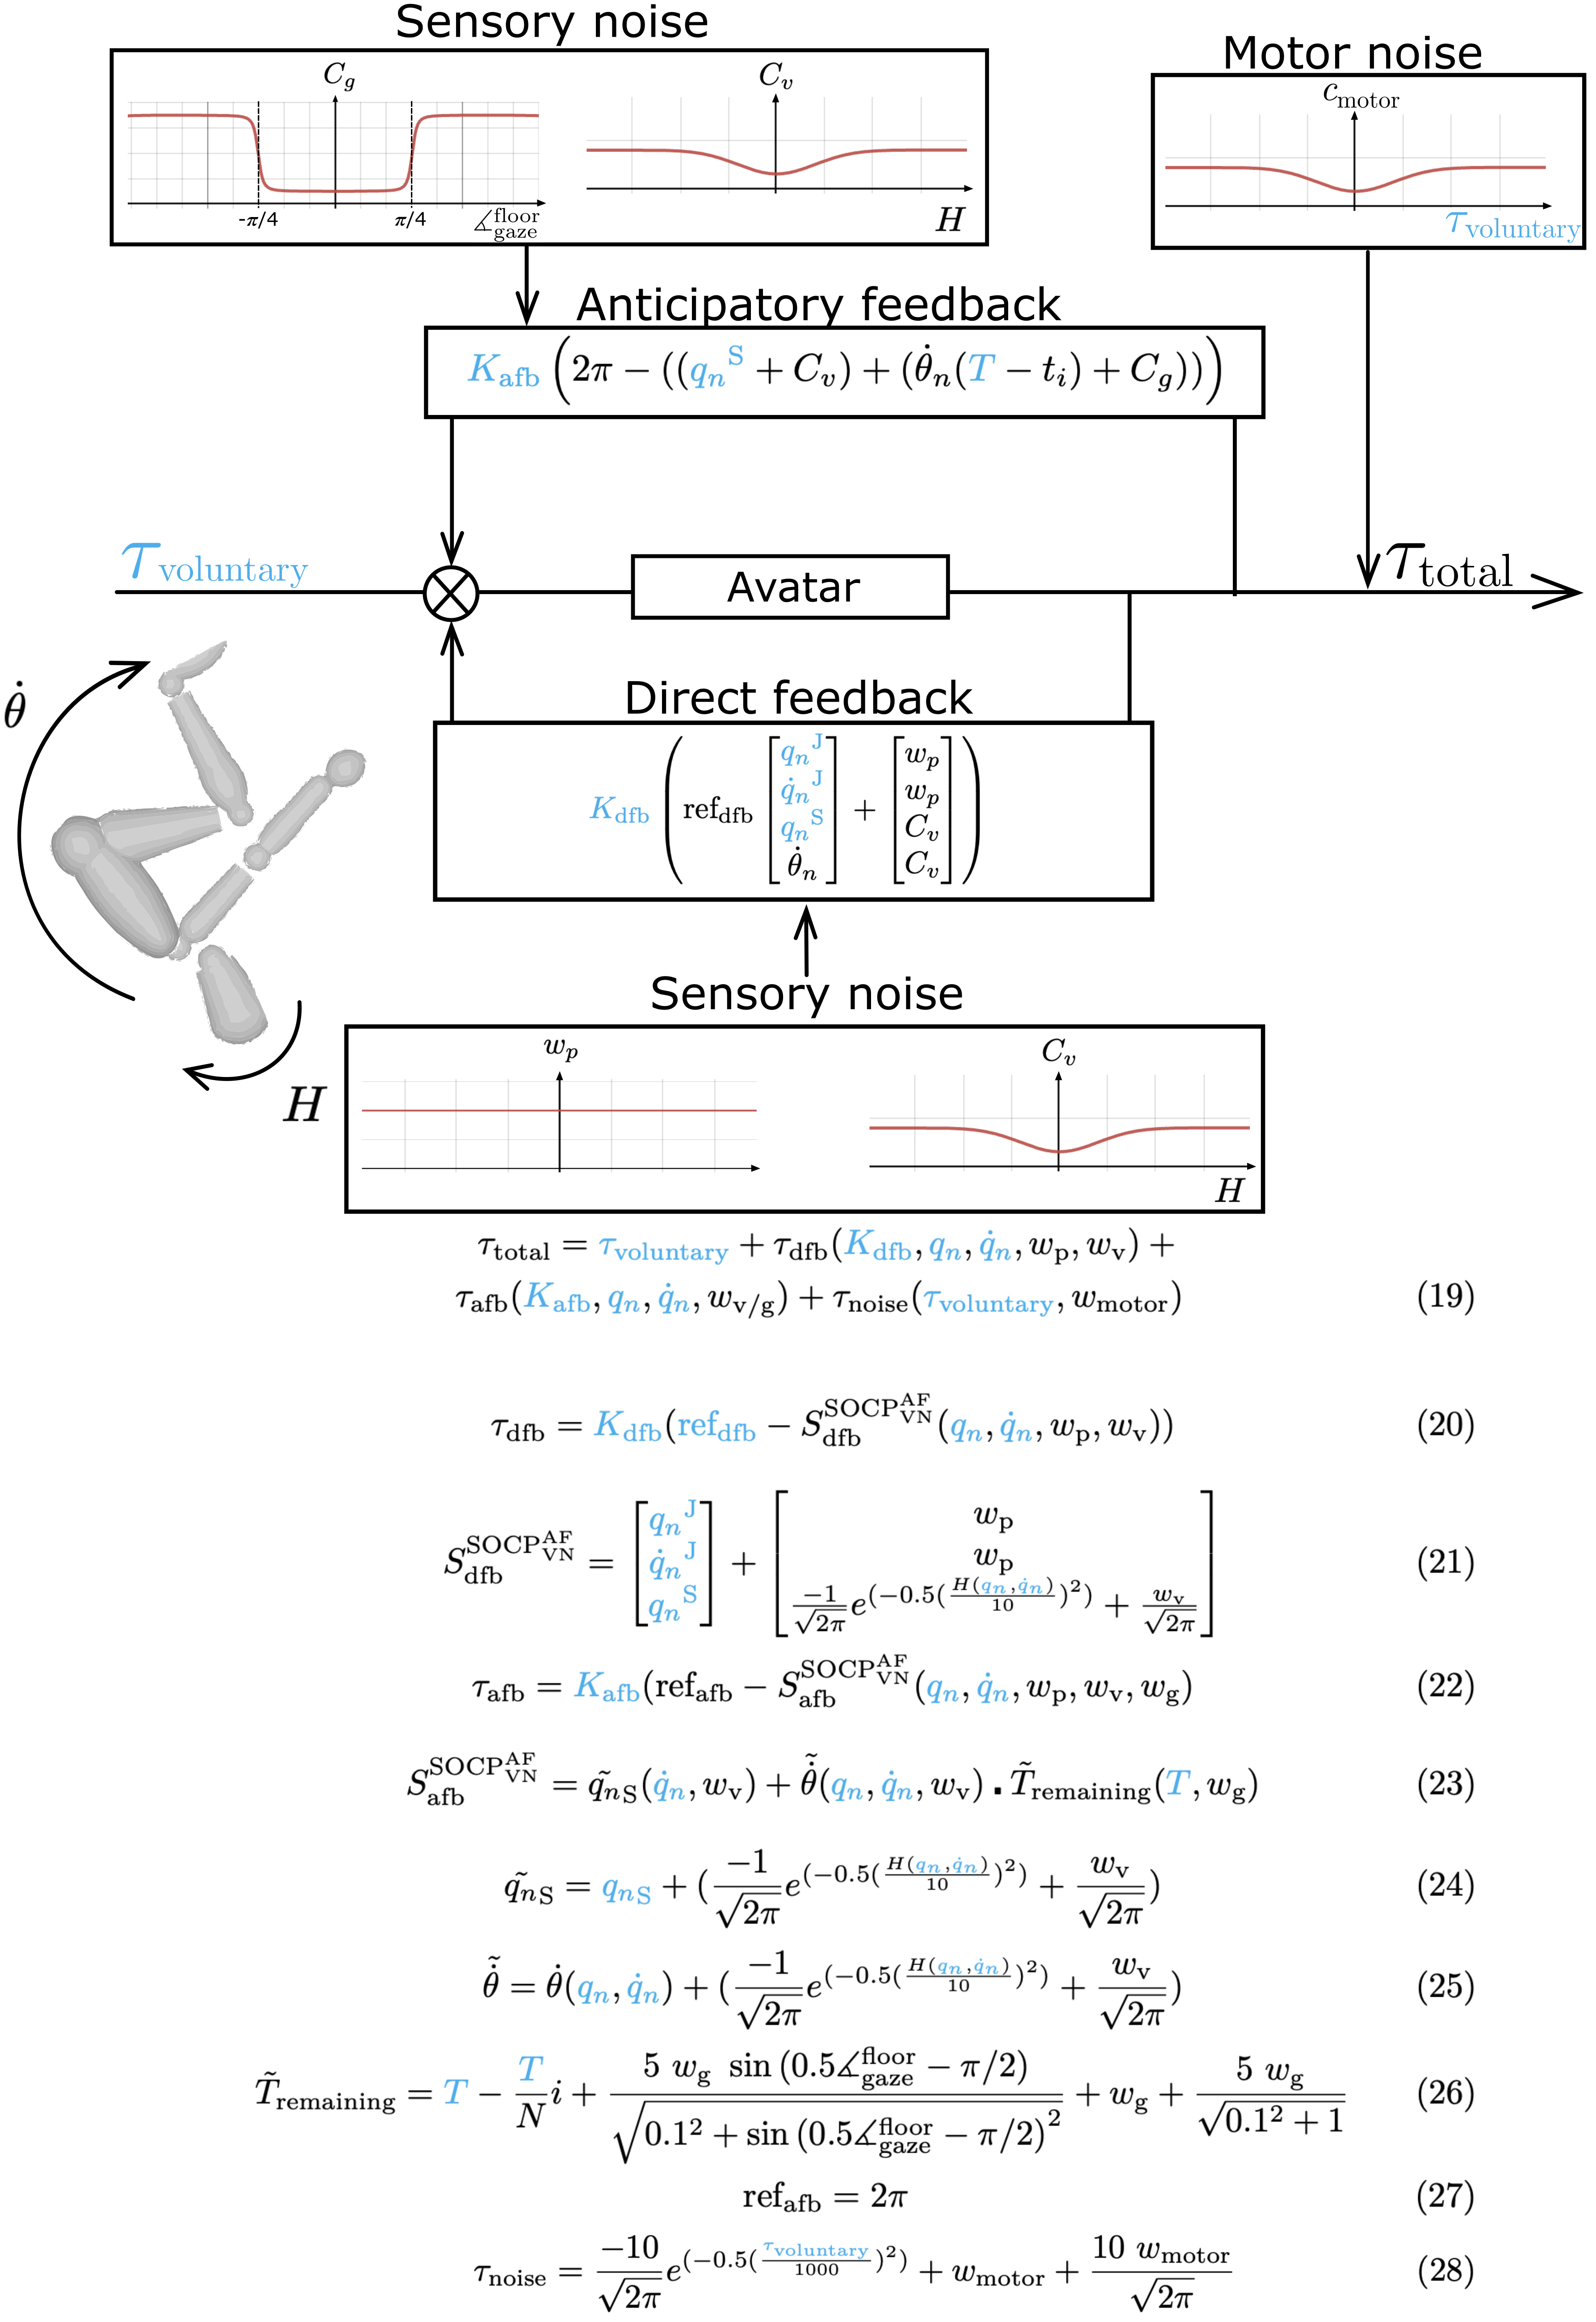
\includegraphics[width=1.0\linewidth]{figures/socp_plus.png}
\caption{A schematic and mathematical representation of the torques applied to the joints in the SOCP$_{\text{VN}}^{\text{AF}}$ implementation. The $\tilde{.}$ symbol represents corrupted sensory information.}
\label{fig:socp_plus}
\end{figure}


\subsection{Optimization problem implementation}
\setcounter{equation}{26}
The optimization problems were formulated using direct multiple-shooting.
The total duration of the aerial phase of the backward somersault ($\textcolor{gray}{T}$) was included in the optimal control problem as an optimization variable.
The movement time was discretized into 16 equal-duration time intervals.
Continuity constraints ($g_{\text{DMS}}$) were imposed at each time interval transitions to ensure the joint generalized coordinates and velocities from each episode were continuous throughout the entire movement:
%
\begin{equation}
g_{\text{DMS}} :  
\begin{bmatrix}
\textcolor{gray}{q_{j+1}} \\ 
\textcolor{gray}{\dot{q}_{i+1}}
\end{bmatrix} - \int_{t_i}^{t_{i+1}}{
\begin{bmatrix}
\textcolor{gray}{\dot{q}_i} \\ 
F(\textcolor{gray}{q_i}, \textcolor{gray}{\dot{q}_i}, \tau_{{\text{total}}_i})
\end{bmatrix}
dt} = 0
\end{equation}

Specific constraints were also added to ensure the athlete avatar landed the backward somersault on the floor ($g_1$) with its center of mass (CoM) over its forefeet ($g_2$).
%
\begin{eqnarray}
g_1 : P(\textcolor{gray}{q_i}, \textcolor{gray}{T})_z = 0 \\
g_2: P(\textcolor{gray}{q_i}, \textcolor{gray}{T})_y - CoM(\textcolor{gray}{q_i}, \textcolor{gray}{T})_y = 0
\end{eqnarray}
%
\noindent where $P$ is the position of the forefoot marker.
for all simulations, an initial standing posture with extended body and arms upward, vertical velocity ($2~m/s$) and somersault velocity ($450\degree/s$) were imposed to match real athletes' take-off position.
For the stochastic version, an additional constraint was added so that the reference ($\textcolor{gray}{ref}$) sensory input was equal to the mean sensory input ($S$) over all episodes.
\begin{equation}
g_3: \textcolor{gray}{ref_i} - \overline{S}(\textcolor{gray}{q_i}, \textcolor{gray}{\dot{q}_i}, t_i) = 0
\end{equation} 

It is worth noticing that the backward somersault is a highly constrained movement, limiting the number of viable techniques.
This movement was chosen as the sensorimotor strategies involved in it are well established \cite{bardy1998body, heinen2011evidence, davlin2004gymnasts, luis2008visual, natrup2021gaze}. 


The cost function was composed of multiple terms to generate the best acrobatic movement, while ensuring numerical stability.
The main objective of the stochastic optimal control problems was to minimize landing instability, defined as the variability in center of mass position, center of mass velocity, and body angular velocity at landing.
\begin{eqnarray}
\phi_1 = \num{1e+4}~\sum_{n}^{episodes}{(CoM(\textcolor{gray}{q_n}, t_i)_y -\overline{CoM(\textcolor{gray}{q}, t_i)})_y^2} +\\
 \num{1e+4}~\sum_{n}^{episodes}{(\dot{CoM}(\textcolor{gray}{q_n}, t_i)_y -\overline{\dot{CoM}(\textcolor{gray}{q}, t_i)})_y^2} +\\
 \num{1e+4}~\sum_{n}^{episodes}{(L(\textcolor{gray}{q_n}, \textcolor{gray}{\dot{q}_n}, t_i)/I(q_n, t_i) -\overline{L(\textcolor{gray}{q}, \textcolor{gray}{\dot{q}}, t_i)/I(\textcolor{gray}{q}, t_i)})^2}
\end{eqnarray}
\noindent where $n$ is the number of the episode, $L$ is the whole body angular momentum, and $I$ is the whole body transverse moment of inertia.
An additional term was added to minimize the expected efforts needed to complete the acrobatics:
\begin{equation}
\phi_2 = 0.01~\int_{0}^{\textcolor{gray}{T}}{\tau_{\text{total}}^2~dt}
\end{equation}
Another term minimized the expected rate of change in effort to promote a psychophysiological motor command:
\begin{equation}
\phi_3 = 0.01~\int_{0}^{\textcolor{gray}{T}}{{\dot{\tau}_{\text{total}}}^2~dt}
\end{equation}
Regularization terms were also added to ensure that the feedback gains, the rate of change of the feedback gains, and the total movement duration remained within acceptable ranges:
\begin{eqnarray}
\phi_4 = \num{1e-5}~\int_{0}^{\textcolor{gray}{T}}{\textcolor{gray}{K}^2~dt} \\
\phi_5 = 1~\int_{0}^{\textcolor{gray}{T}}{\dot{\textcolor{gray}{K}}^2~dt} \\
\phi_6 = 0.01~\textcolor{gray}{T}
\end{eqnarray}
The weights of the objective terms were manually fine-tuned to achieve a solution that \textit{i)} looks realistic enough and \textit{ii)} had enough variability in the SOCP implementation to leave room for improvement in the other implementations, but not so much as to compromise convergence.


The complete approximate stochastic optimal control transcription was as follows:
\begin{equation}
\begin{array}{ll@{}ll}
\underset{\textcolor{gray}{q}, \textcolor{gray}{\dot{q}}, \textcolor{gray}{\tau_{\text{voluntary}}}, \textcolor{gray}{\text{ref}}, \textcolor{gray}{K}, \textcolor{gray}{T}}{\min} & \phi_1 + \phi_2 + \phi_3 + \phi_4 + \phi_5 + \phi_6 \\
\text{~~~~~~~~~s.t.} & g_{\text{DMS}}=0 \\
            & g_1 = 0 \\
            & g_2 = 0 \\
            & g_3 = 0 \\
            & \textcolor{gray}{q} \in \mathcal{Q} \\
            & \textcolor{gray}{\dot{q}} \in \dot{\mathcal{Q}} \\
            & \textcolor{gray}{\tau_{\text{voluntary}}} \in \mathcal{\tau} \\
            & \textcolor{gray}{\text{ref}} \in \mathcal{R} \\
            & \textcolor{gray}{K} \in \mathcal{K} \\
            & \textcolor{gray}{T} \in \mathcal{T} \\
\end{array}
\end{equation}

\subsection{Comparison of the optimal solutions}
The optimal kinematics from the problem transcriptions were compared using statistical parametric mapping (SPM1D) \cite{pataky2012one}.
The optimal joint torques were split into their components to analyze the contribution of open-loop control ($\textcolor{gray}{\tau_{\text{voluntary}}}$), joint damping, direct feedback control ($\tau_{\text{dfb}}$), and anticipatory feedback control ($\tau_{\text{afb}}$).
The head rotation velocity and eye orientation were analyzed to extract sensory acquisition strategies from the optimal acrobatic techniques.

\section{Results}\label{sec:results}

\subsection{Landing variability performance}

The main performance objective of the task considered in this study was to minimize landing variability ($\phi_1$), measured as the sum of the CoM horizontal position, CoM horizontal velocity, and body angular velocity variances at the end of the movement.
All stochastic implementations outperformed the deterministic one in terms of landing variability (OCP: 14115.4, SOCP: 62.2, SOCP$_{\text{VN}}$: 27.5, SOCP$^{\text{AF}}$: 21.2,
SOCP$_{\text{VN}}^{\text{AF}}$: 21.2).
The smallest landing variability was achieved with the SOCP$_{\text{VN}}^{\text{AF}}$ implementation, an improvement of more than two orders of magnitude (664.8) compared to the OCP implementation.

\begin{figure}[H]
\centering
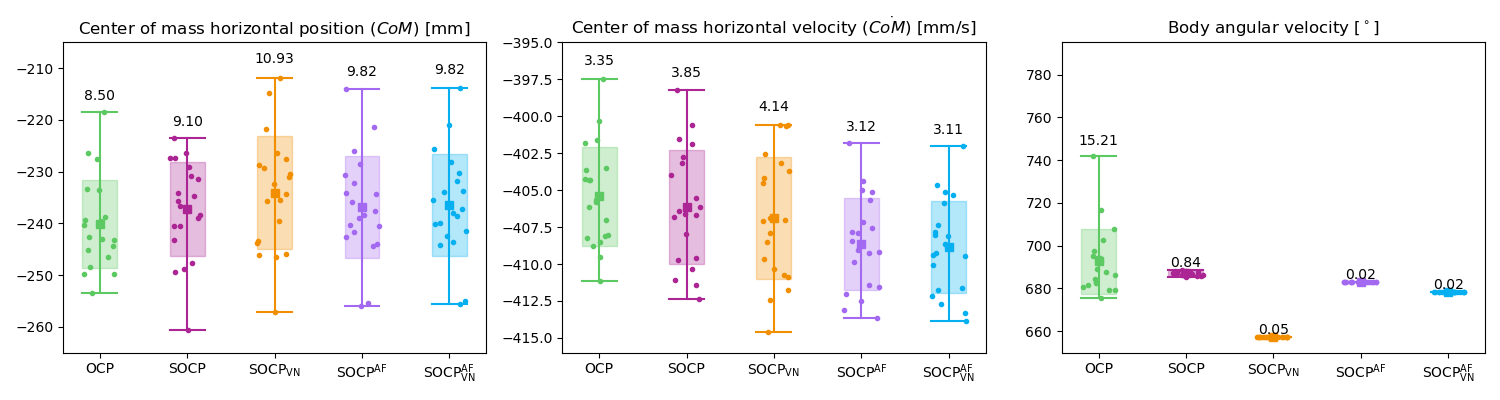
\includegraphics[width=1.0\linewidth]{figures/landing_variability.png}
\caption{The three landing variability components (center of mass horizontal position, center of mass horizontal velocity, and body angular velocity) for the backward somersault generated with the \textcolor{OCP_color}{OCP} (green), \textcolor{SOCP_color}{SOCP} (pink), \textcolor{SOCP_VARIABLE_color}{SOCP$_{\text{VN}}$} (orange), \textcolor{SOCP_FEEDFORWARD_color}{SOCP$^{\text{AF}}$} (purple), and \textcolor{SOCP_plus_color}{SOCP$_{\text{VN}}^{\text{AF}}$} (blue) implementations. The value for each episode is depicted with a dot, the mean over all episodes is depicted with a square, the standard deviation range is depicted with a box, and the standard deviation is written above the box plot.}
\label{fig:landing_variability}
\end{figure}


\subsection{Kinematics}

An optimal solution (Fig.~\ref{fig:kinograms}) was reached for each implementation (\textcolor{OCP_color}{OCP}, \textcolor{SOCP_color}{SOCP}, \textcolor{SOCP_VARIABLE_color}{SOCP$_{\text{VN}}$} \textcolor{SOCP_FEEDFORWARD_color}{SOCP$^{\text{AF}}$}, \textcolor{SOCP_plus_color}{SOCP$_{\text{VN}}^{\text{AF}}$}).
The convergence time considerably increased for the stochastic implementations (few weeks) compared to the deterministic implementation (few seconds).
The duration of the acrobatic was similar across implementations (OCP: 0.4048~s, SOCP: 0.4047~s, SOCP$_{\text{VN}}$: 0.4049~s, SOCP$^{\text{AF}}$: 0.4040~s, SOCP$_{\text{VN}}^{\text{AF}}$: 0.4030~s). 
The implementation significantly influenced the optimal kinematics (Fig.~\ref{fig:kinematics}).
All joint angle time series were significantly different between implementations for at least 59\% of the movement.
Notably, the knees were kept extended longer, and the initial hip flexion was less pronounced in the deterministic version (OCP).
The landing posture was similar across implementations except for the shoulder angle.


\begin{figure}[H]
\centering
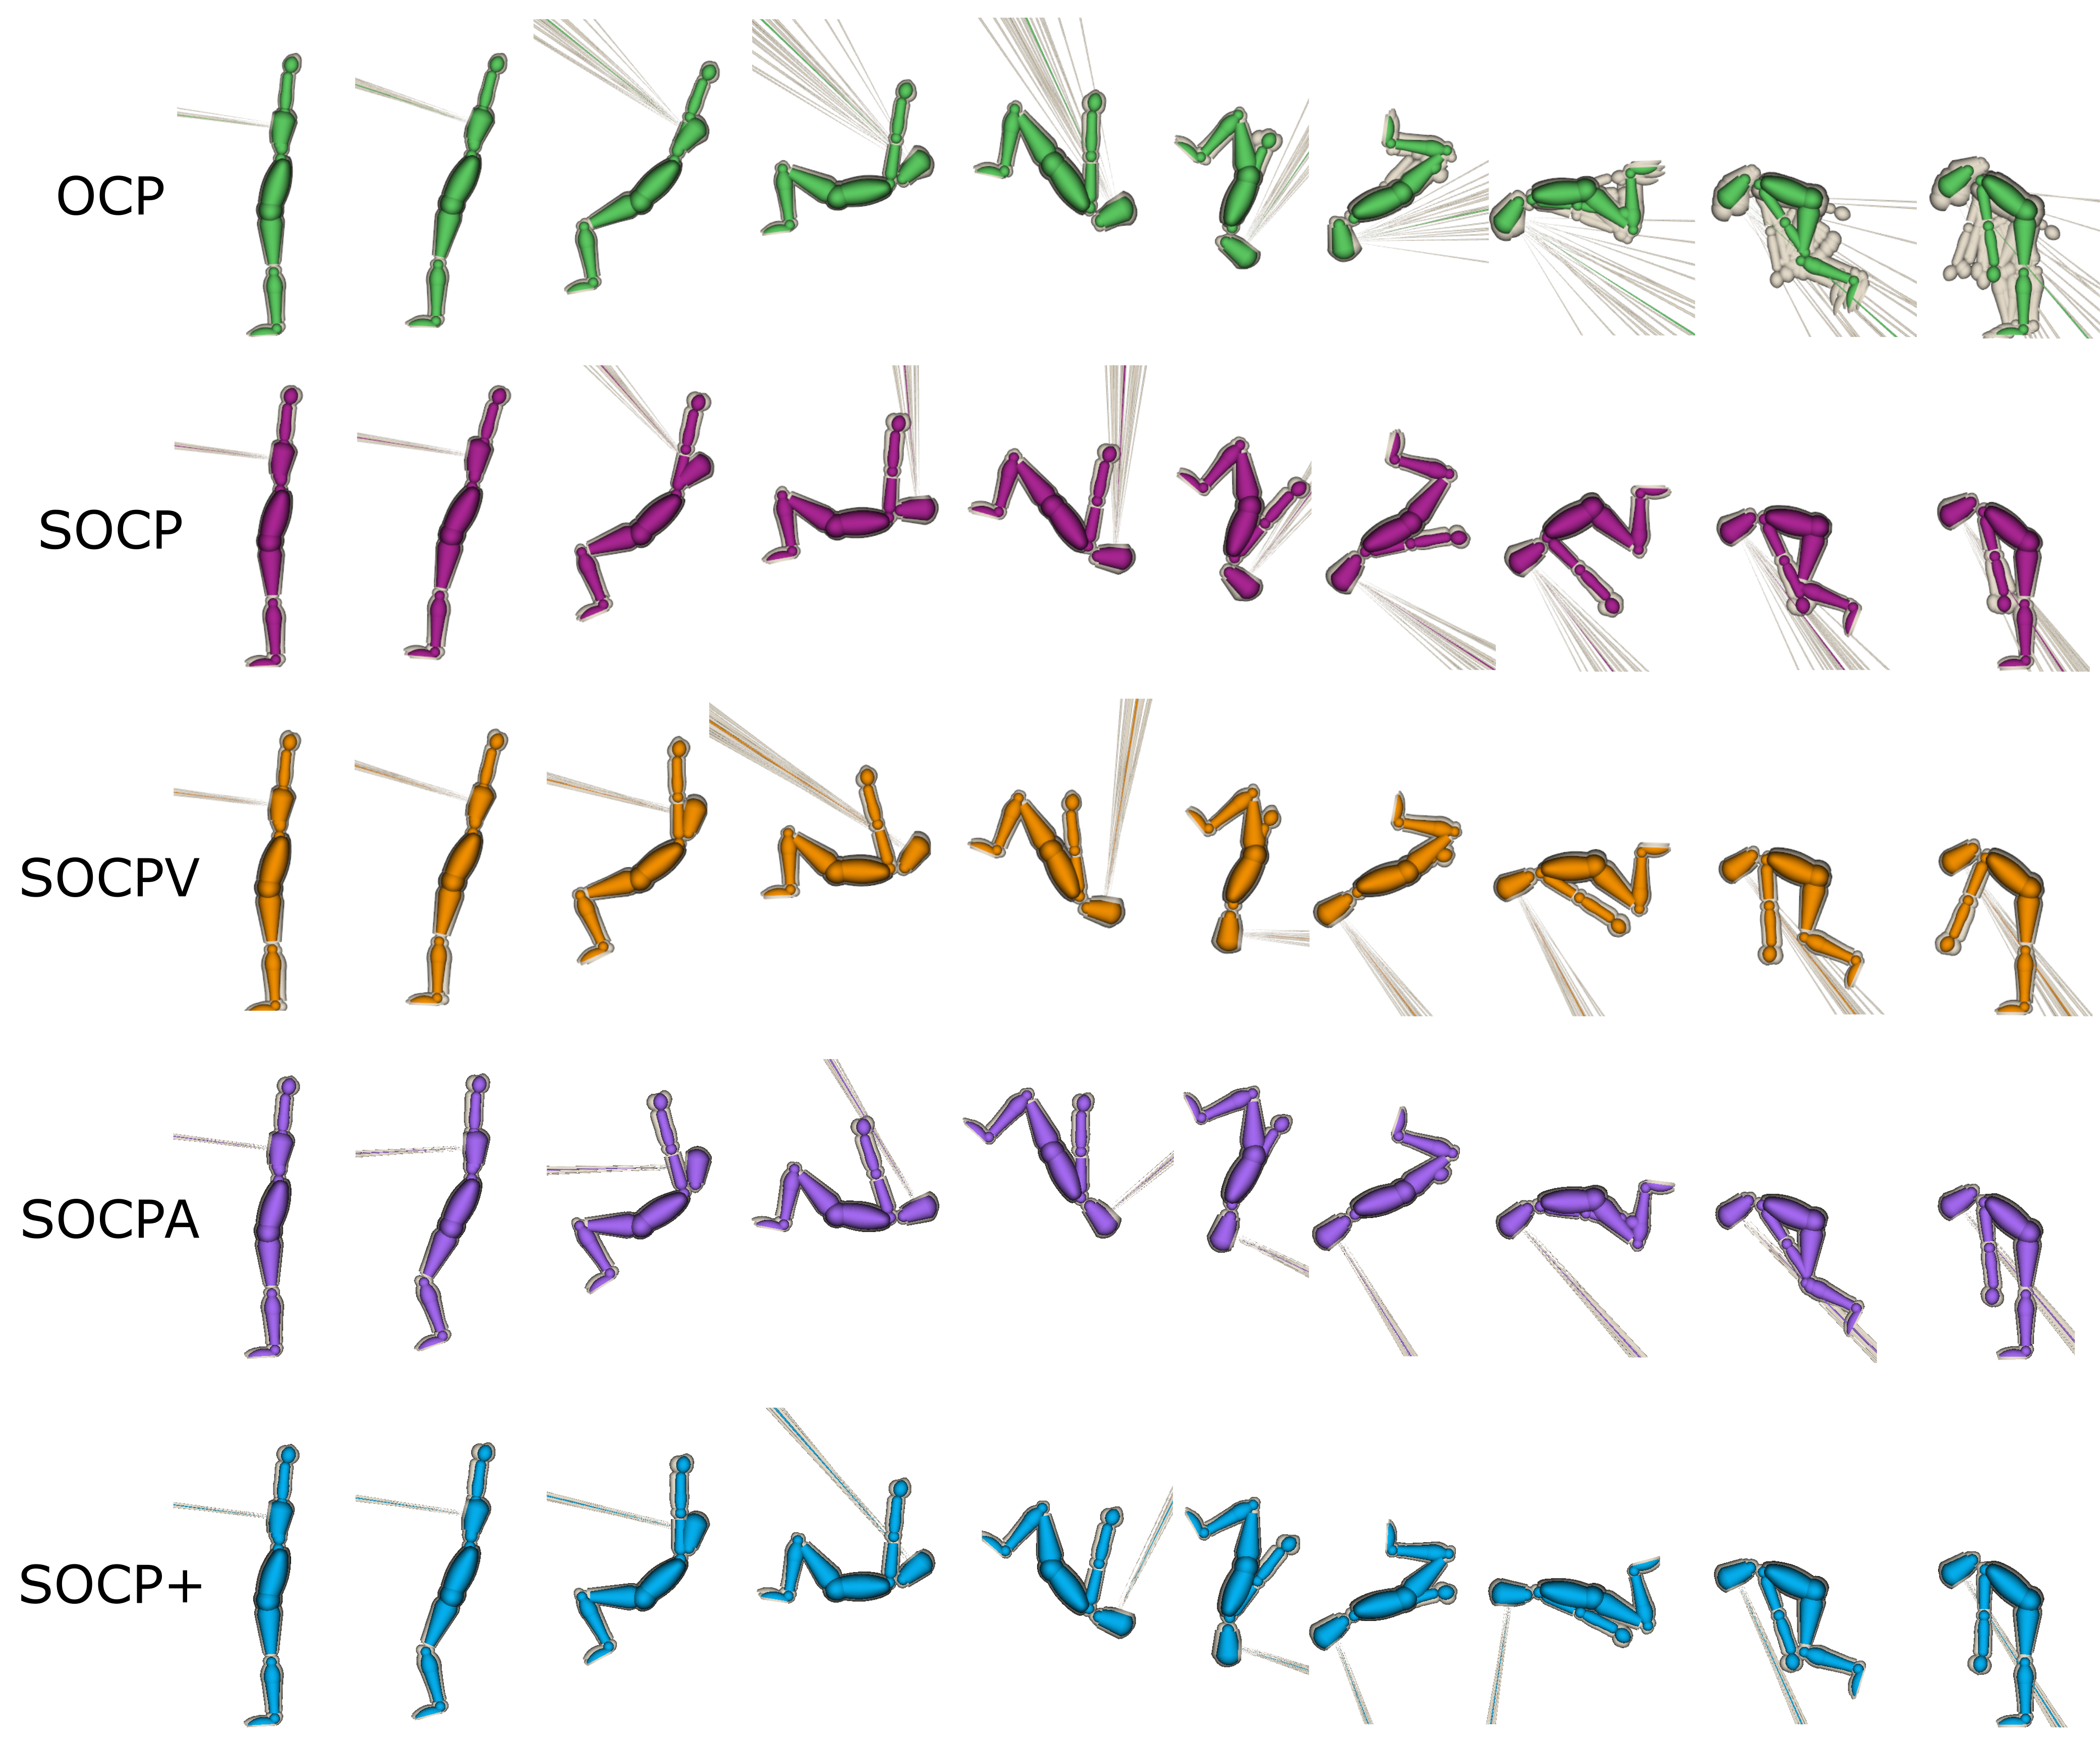
\includegraphics[width=1.0\linewidth]{figures/kinograms.png}
\caption{Animation of the optimal kinematics for the backward somersault generated with the OCP (\textcolor{OCP_color}{green}), SOCP (\textcolor{SOCP_color}{pink}), SOCP$_{\text{VN}}$ (\textcolor{SOCP_VARIABLE_color}{orange}), SOCP$^{\text{AF}}$ (\textcolor{SOCP_FEEDFORWARD_color}{purple}), and SOCP$_{\text{VN}}^{\text{AF}}$ (\textcolor{SOCP_plus_color}{blue}) implementations. The grayed avatars represent the optimal joint angles for each episode (except for the OCP version, where they represent a noisy reintegration of the deterministic optimal solution), and colored avatars represent the mean optimal joint angles across episodes.}
\label{fig:kinograms}
\end{figure}

\begin{figure}[H]
\centering
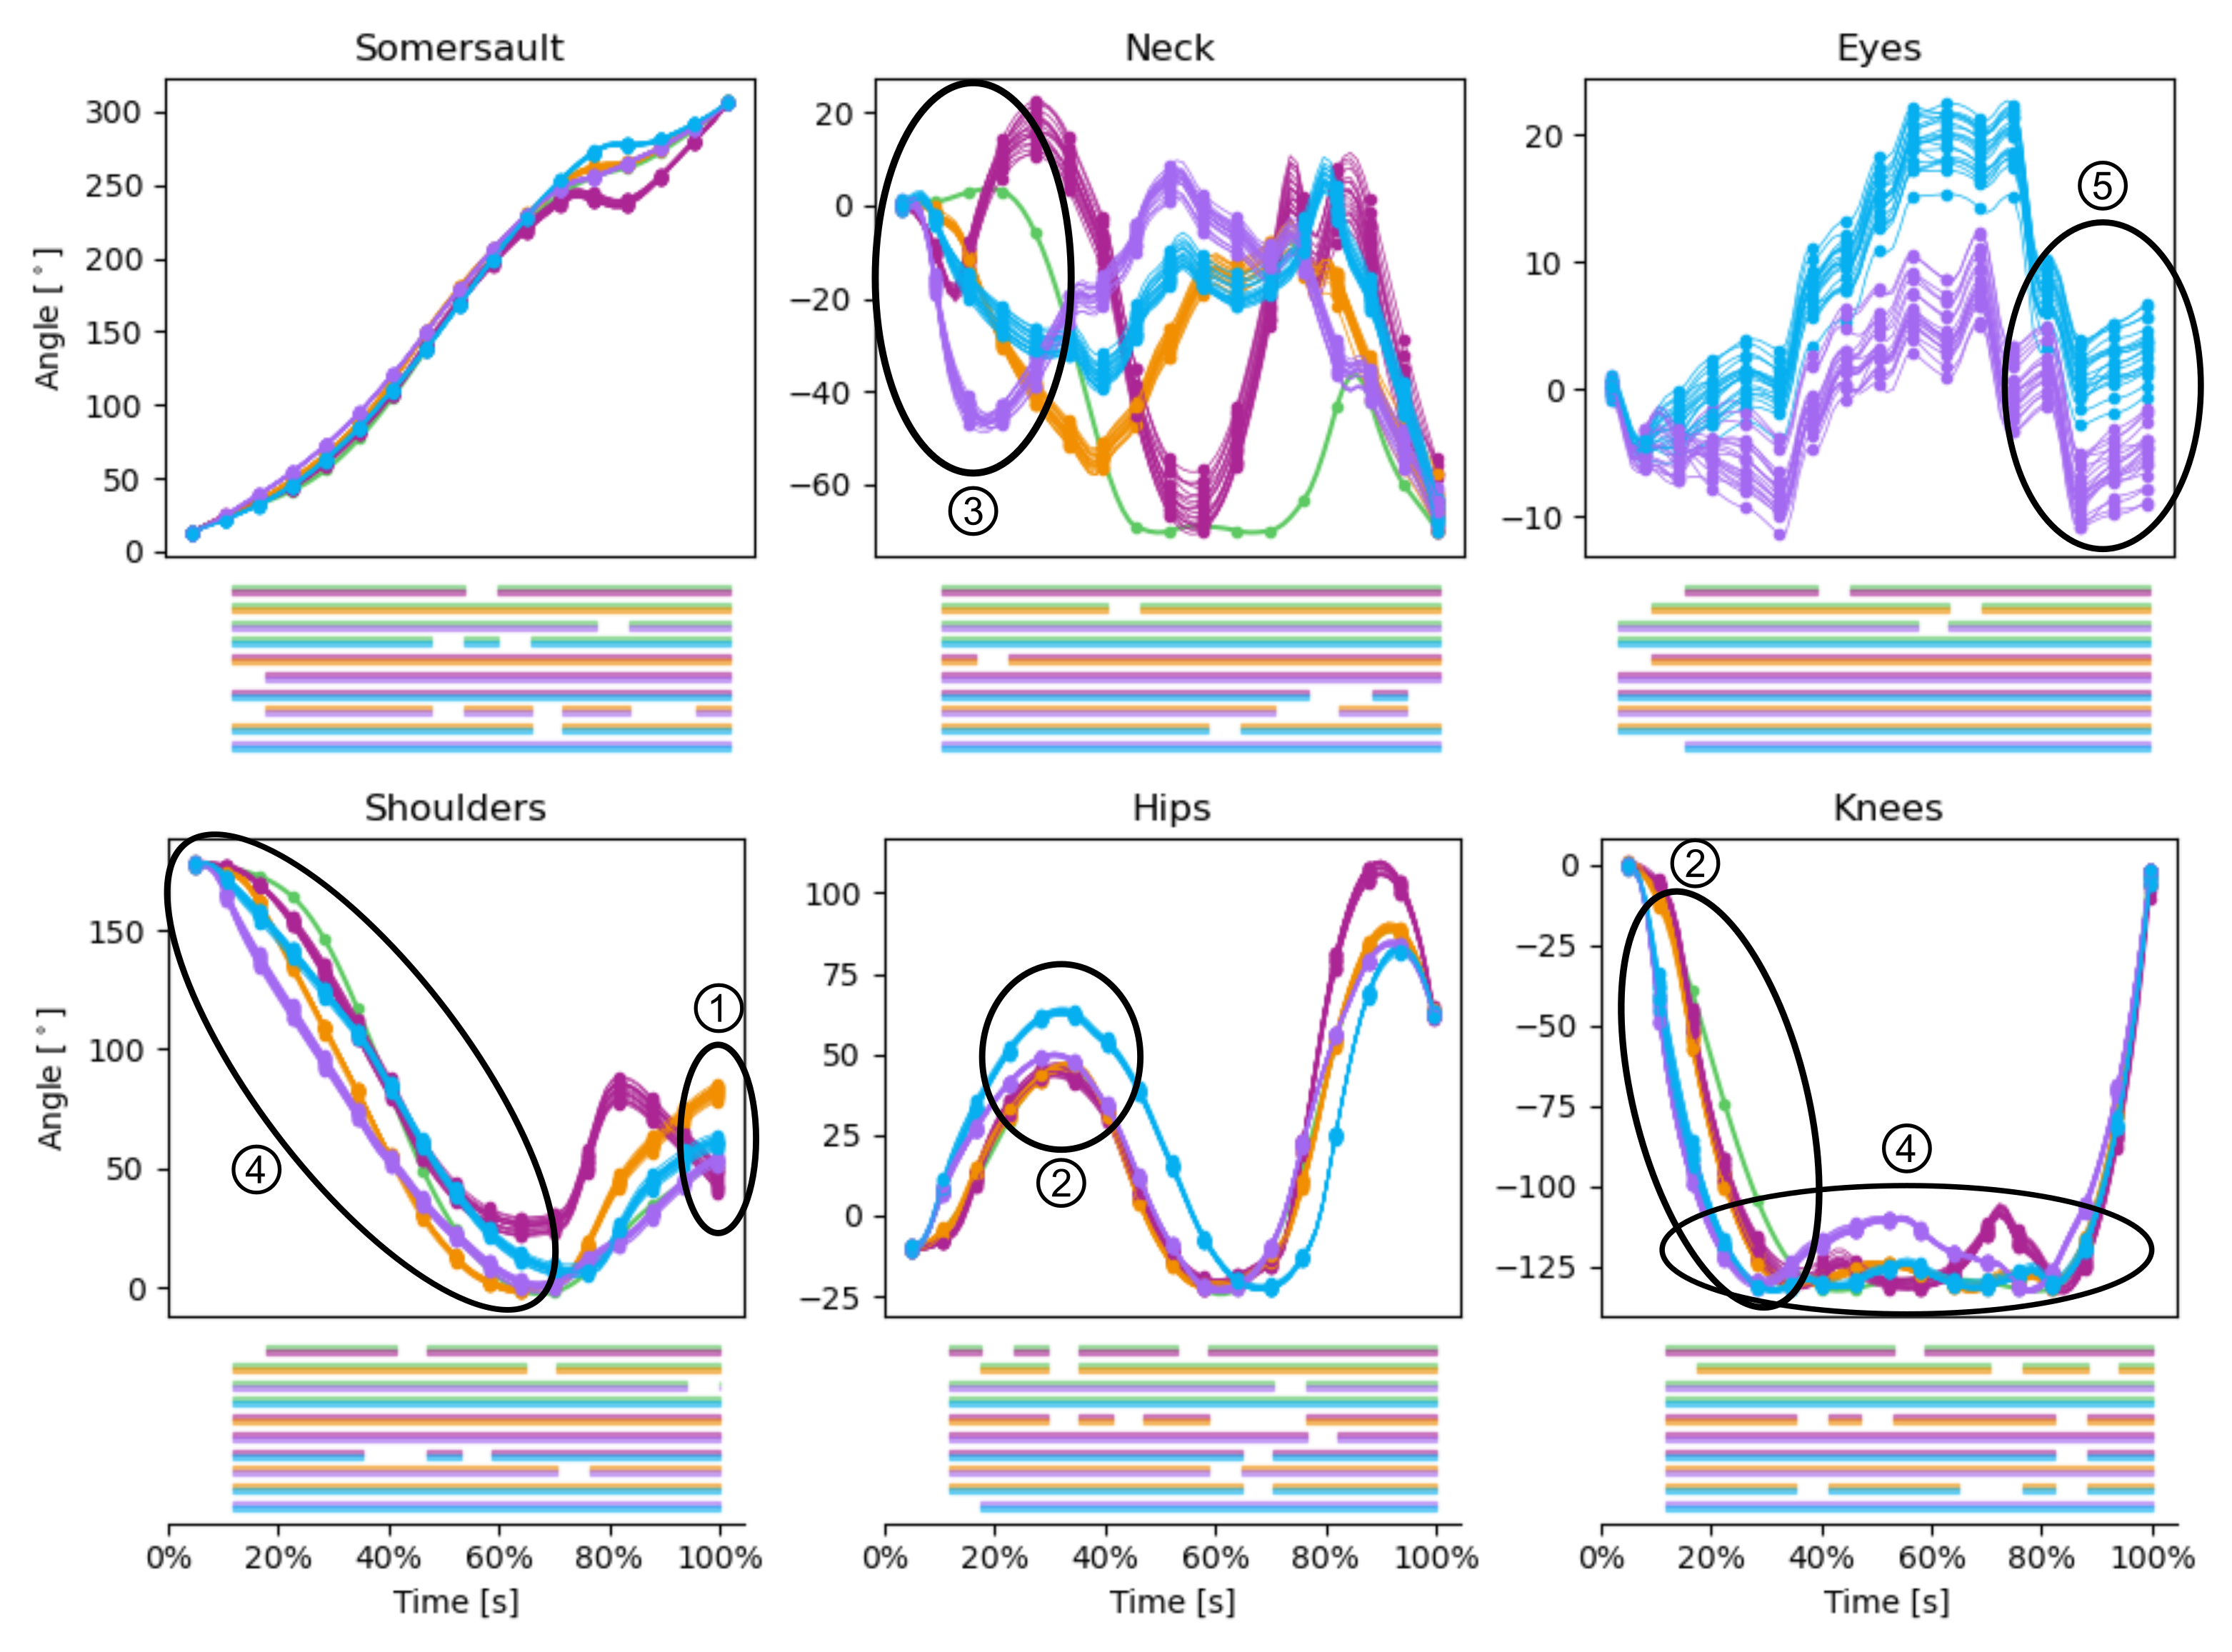
\includegraphics[width=1.0\linewidth]{figures/kinematics.png}
\caption{Optimal kinematics for the backward somersault generated with the OCP (\textcolor{OCP_color}{green}), SOCP (\textcolor{SOCP_color}{pink}), SOCP$_{\text{VN}}$ (\textcolor{SOCP_VARIABLE_color}{orange}), SOCP$^{\text{AF}}$ (\textcolor{SOCP_FEEDFORWARD_color}{purple}), and SOCP$_{\text{VN}}^{\text{AF}}$ (\textcolor{SOCP_plus_color}{blue}) implementations. The dual-coloured bars below the graphs represent the time intervals during which each pair of techniques was significantly different. Meaningful kinematic differences are highlighted using circled numbers for reference throughout the discussion.}
\label{fig:kinematics}
\end{figure}


\subsection{Motor strategies}

The motor command differed between the different implementations (Fig.~\ref{fig:torques_contributions}~a)).
The total torque actuation (integral of the absolute total torque) was larger in the deterministic (OCP: 136.81~Nm.s) than in the stochastic (SOCP: 79.28~Nm.s, SOCP$_{\text{VN}}$: 23.83~ Nm.s, SOCP$^{\text{AF}}$: 29.43~Nm.s, SOCP$_{\text{VN}}^{\text{AF}}$: 36.77~Nm.s) transcriptions.
\comEC{� discuter, OCP force toujours contre l'effet centrifuge j'ai l'impression. Mon guess c'est que c'est un minimum local et que le fait d'optimiser plusieurs mod�les � la fois en stochastique a un effet multi-start qui permet de sortir de ce minimum local. Mais je suis pas assez certaine pour en discuter ici :/. Cost: (OCP: 331.25, SOCP: 4928.34, SOCP$_{\text{VN}}$: 106.26, SOCP$^{\text{AF}}$: 98.52, SOCP$_{\text{VN}}^{\text{AF}}$: 87.70)}
The largest torque contribution came from the open-loop (98.97\%) for the OCP implementation, from direct feedback (65.15\%) for the SOCP implementation, from direct feedback (58.78\%) for the SOCP$_{\text{VN}}$ implementation, from open-loop (38.80\%) and anticipatory feedback (38.38\%) for the SOCP$^{\text{AF}}$ implementation, and from open-loop (39.51\%) and anticipatory feedback (35.75\%) for the SOCP$_{\text{VN}}^{\text{AF}}$ implementation (Fig.~\ref{fig:torques_contributions}~b)).

\begin{figure}[H]
\centering
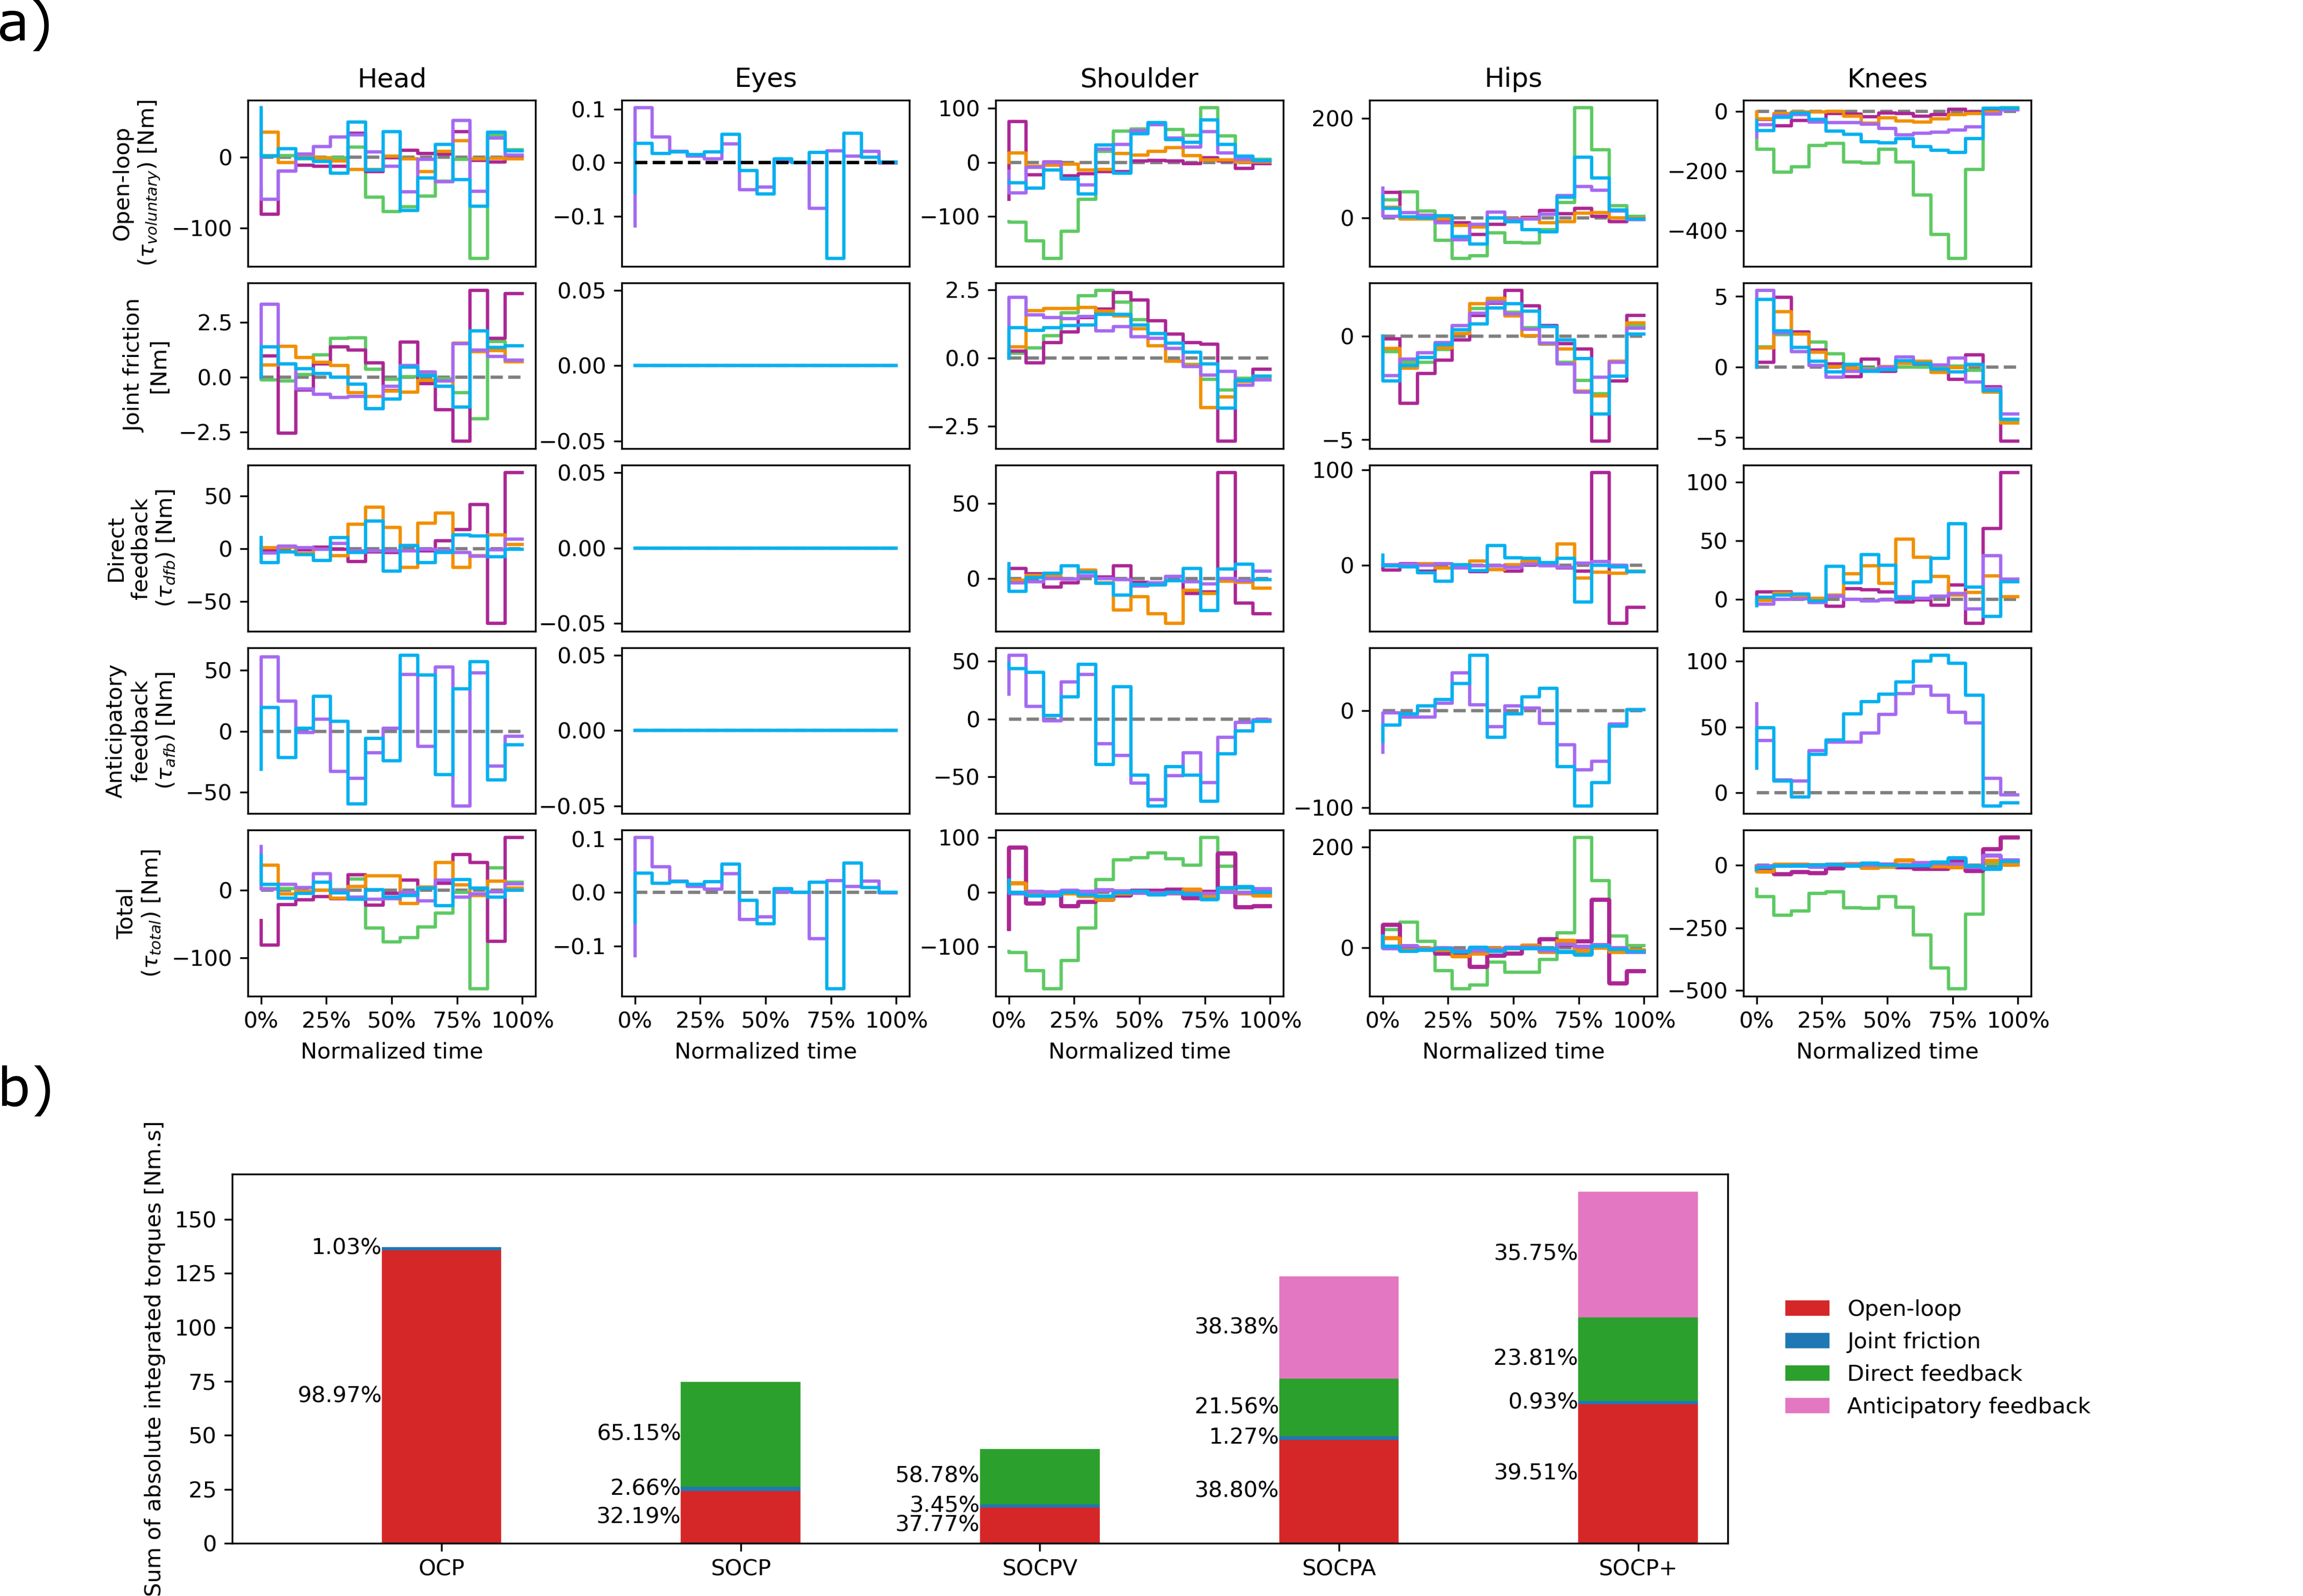
\includegraphics[width=1.0\linewidth]{figures/torques_contributions.png}
\caption{a) Each component of the motor command for the backward somersault generated with the \textcolor{OCP_color}{OCP} (green), \textcolor{SOCP_color}{SOCP} (pink), \textcolor{SOCP_VARIABLE_color}{SOCP$_{\text{VN}}$} (orange), \textcolor{SOCP_FEEDFORWARD_color}{SOCP$^{\text{AF}}$} (purple), and \textcolor{SOCP_plus_color}{SOCP$_{\text{VN}}^{\text{AF}}$} (blue) implementations. The total torque used to actuate the avatar is presented on the last row. For the stochastic implementations, only the means of the joint damping, direct feedback, and anticipatory feedback are presented for clarity. b) The sum of the absolute value of the joint torques integrated for each component of the motor command: Open-loop control (red), joint damping (blue), direct feedback (green), and anticipatory feedback (pink).}
\label{fig:torques_contributions}
\end{figure}

\subsection{Sensory acquisition strategies}

For all implementations, the feedback gains decreased shortly before landing (Fig.~\ref{fig:sensory_strategies} a)).
The hip feedback gains were maximal when fully tucked and fully extended during the middle part of the acrobatics.
When anticipatory feedback was available, its gain on the knees DoF reached the maximum bound (saturated) for most of the acrobatics.
The mean absolute eye orientation was smaller in the SOCP$_{\text{VN}}^{\text{AF}}$ (77.56\degree) than in the SOCP$_{\text{VN}}$ (80.34\degree), especially at the end of the acrobatics, when visual anticipatory feedback is available.

\begin{figure}[H]
\centering
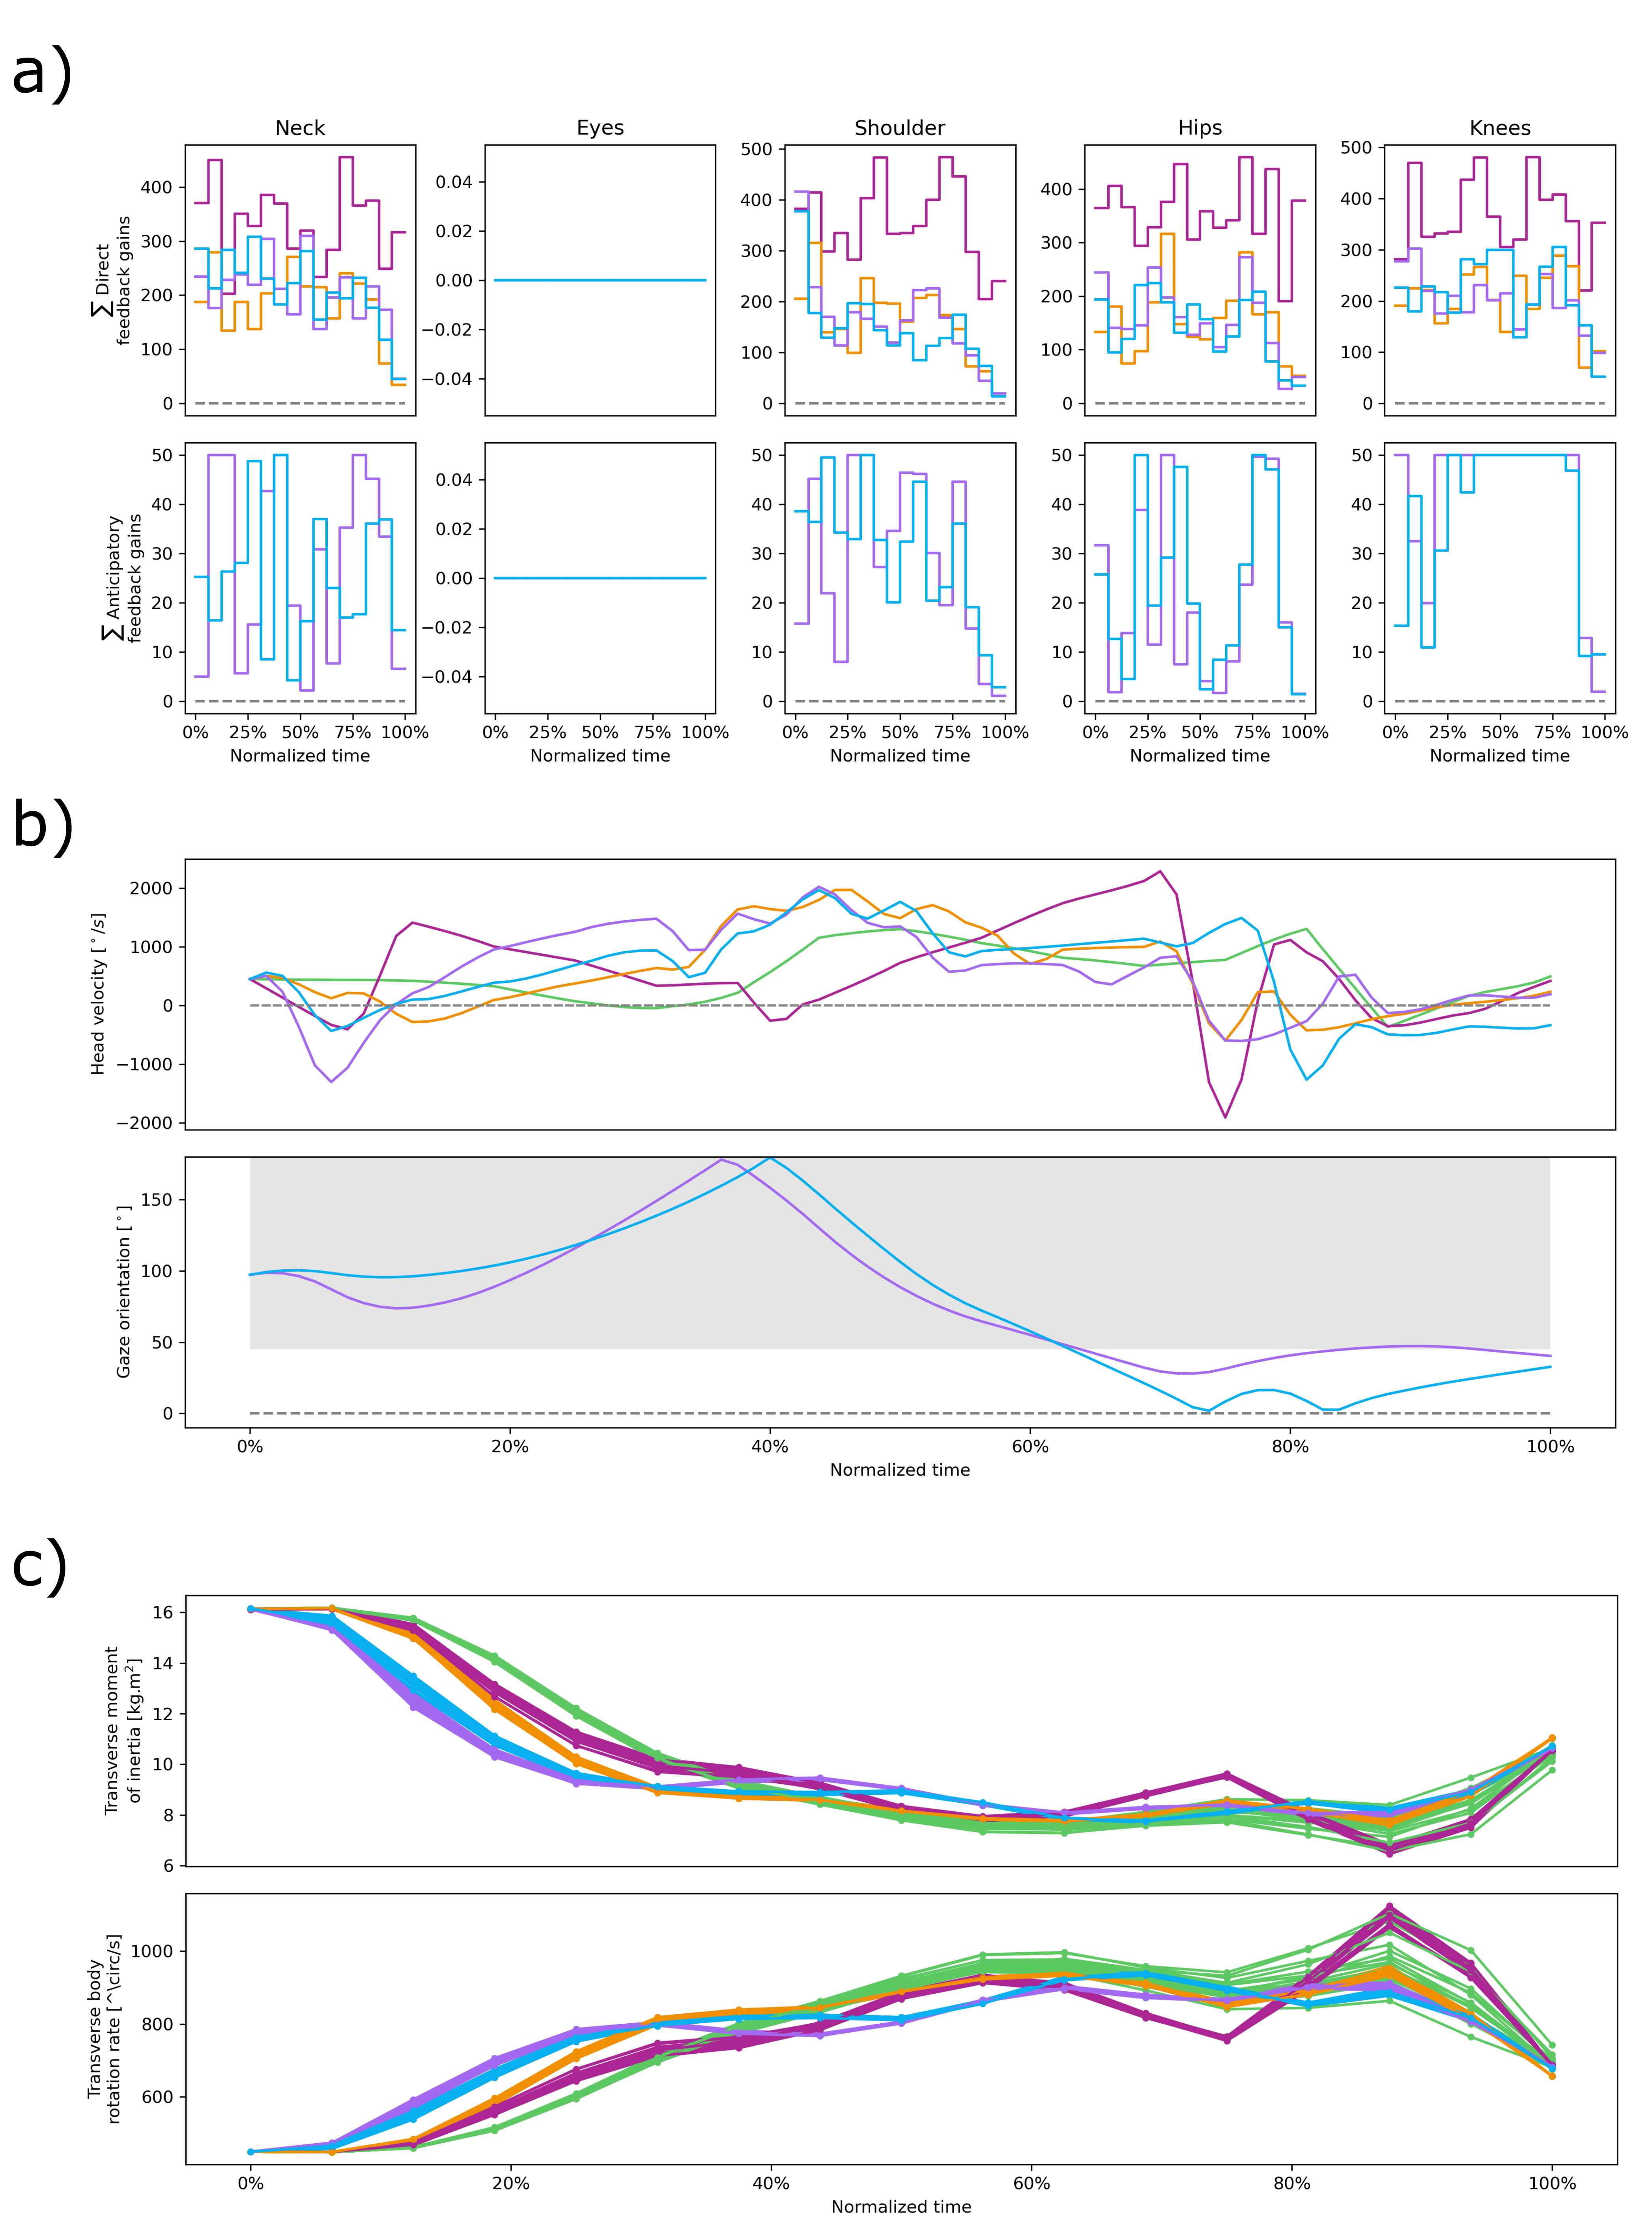
\includegraphics[width=1.0\linewidth]{figures/sensory_strategies.png}
\caption{a) The feedback gains (k) and c) the transverse moment of inertia and body rotation rate ($\dot{\theta}$) for the backward somersault generated with the \textcolor{OCP_color}{OCP} (green), \textcolor{SOCP_color}{SOCP} (pink), \textcolor{SOCP_VARIABLE_color}{SOCP$_{\text{VN}}$} (orange), \textcolor{SOCP_FEEDFORWARD_color}{SOCP$^{\text{AF}}$} (purple), and \textcolor{SOCP_plus_color}{SOCP$_{\text{VN}}^{\text{AF}}$} (blue) implementations. b) The head angular velocity in the global reference frame and the angle between the vertical and the eye orientation of the mean technique for the \textcolor{SOCP_FEEDFORWARD_color}{SOCP$^{\text{AF}}$} (purple), and \textcolor{SOCP_plus_color}{SOCP$_{\text{VN}}^{\text{AF}}$} (blue) implementations.}
\label{fig:sensory_strategies}
\end{figure}


\section{Discussion}\label{sec:discussion}

Optimal techniques were generated for the aerial phase of the backward somersault using a deterministic transcription of an optimal control problem and four variations of stochastic transcriptions. 
The landing conditions were compared between implementation to test our hypothesis that using direct sensory feedback would reduce landing variability (H1) and that using anticipatory sensory feedback would further reduce landing variability (H2).
The first hypothesis was confirmed as the OCP transcription, the only implementation without direct sensory feedback, had the largest landing variability.
The second hypothesis was also confirmed as the SOCP$^{\text{AF}}$ and SOCP$_{\text{VN}}^{\text{AF}}$, the two only implementations with anticipatory sensory feedback, had the lowest landing variability. 
The kinematics of the optimal solutions were compared between implementation to test our hypothesis that sensorimotor strategies would emerge from implementations considering state-dependent sensory noise (H3) and that the most advanced implementation would generate techniques that more closely resembled the technique used by athletes (H4).
The third hypothesis was confirmed as the SOCP$_{\text{VN}}^{\text{AF}}$ technique presented the two sensorimotor strategies used by athletes: head stabilization (spotting) and stabilizing the gaze on the floor before landing.
The head stabilization strategy was also present in the SOCP$_{\text{VN}}$.
The fourth hypothesis was also confirmed as some features of the technique used by experienced athletes emerged from the SOCP$_{\text{VN}}^{\text{AF}}$ transcription.
Interestingly, the technique generated with the OCP transcription resembled more the technique used by athletes during their learning process.  


\subsection{Landing variability}

As observed in other stochastic simulation studies \citep{van2022approximate, berret2024co}, including uncertainty in the optimal control problem implementation enabled the generation of optimal techniques more robust to motor noise. 
In line with our first hypothesis (H1), all our stochastic implementations (SOCP, SOCP$_{\text{VN}}$, SOCP$^{\text{AF}}$, SOCP$_{\text{VN}}^{\text{AF}}$) outperformed our deterministic implementation (OCP) in terms of landing variability, the main performance indicator in this study.
Furthermore, the SOCP$^{\text{AF}}$ and SOCP$_{\text{VN}}^{\text{AF}}$ simulations exhibited the smallest landing variability, showing that the addition of anticipatory feedback helped increase robustness to motor noise, confirming our second hypothesis (H2).
The beneficial role of anticipatory feedback (also called prospective regulation) during the backward somersault was also suggested by Bardy \& Laurent \cite{bardy1998body}, based on experimental evidence showing that landing variability is increased in darkness (\textit{i.e.}, no vision) conditions.   
The prospective regulation of landing variability in SOCP$^{\text{AF}}$ and SOCP$_{\text{VN}}^{\text{AF}}$ simulations was mainly achieved by making adjustments to the shoulder joint kinematics (Fig.~\ref{fig:kinematics} \circled{1}).
This strategy was also observed in trampolinists, where the upper-limb variability was increased during the last part of the acrobatics to allow reducing the body orientation variability at landing \cite{bourgeois2025motor}.
Modifying the upper-limbs technique offers an efficient way to regulate body rotation velocity by adjusting the moment of inertia, as these segments are less constrained by the acrobatic task ($g_2$: lower-limbs are constrained by the need to keep the center of mass above the feet).
In agreement with the measurement of athletes' variability regulation,  this study suggests that athletes use an internal model to predict their future state and make appropriate anticipatory corrections.


\subsection{Kinematics}

The optimal kinematics generated in this study generally match athletes' technique with flexion and extension of the hips and knees, accompanied by arms lowering \cite{bradley2020comparison, leboeuf2012optimal}.
The kinematic differences between implementations are subtle, yet some of them are meaningful.
Interestingly, the OCP optimal kinematics resembles the technique used by novice gymnasts in their early phase of learning the backward somersault. 
In contrast, the SOCP$_{\text{VN}}^{\text{AF}}$ optimal kinematics resembles the technique used by more experienced gymnasts.
This difference was noticeable in a looser tuck position in the OCP compared to SOCP$_{\text{VN}}^{\text{AF}}$ simulations, as observed in beginners compared to experts in \cite{kikuchi2006kinematical}.
This looser tuck position was caused by a smaller hip flexion and a later knee flexion (Fig.~\ref{fig:kinematics} \circled{2}). 
In addition, the OCP kinematics presented a neck extension during the elevation phase (Fig.~\ref{fig:kinematics} \circled{3}). 
This neck elevation is often noticible in the technique of novice athletes as early as during the propulsion phase.
% Seul article o� on voit ce lanc� de t�te, mais athl�te charact�ris� d'"�lite" --' : IDENTIFICATION OF INTERNAL LOADS AT THE SELECTED JOINTS DURING PERFORMANCE OF A BACKWARD SOMERSAULT
In the current study, the propulsion phase was not modeled, leading to only a subtle neck extension.
In contrast, the SOCP$_{\text{VN}}^{\text{AF}}$ presented neck flexion, stabilizing their head (see Sec.~\ref{sec:head_stabilization} for further discussion of head stabilization).
This discrepancy is also analogous to an athlete's behaviour modification through the learning process.
Natrup et al. \cite{natrup2021gaze} observed that less experienced athletes presented a neck extension and more experienced athletes did not during a backward somersault with a twist on the trampoline.
In continuation of previous findings \cite{harris1998signal, todorov2002optimal}, this study suggests that athletes learn to adapt their motor strategy to account for their own motor variability.


\subsection{Head stabilization strategy}\label{sec:head_stabilization}
Berthoz \& Pozzo \cite{berthoz1994head} highlighted that athletes exhibit two periods of head stabilization: during the elevation phase after take off and in preparation for landing.
These two periods are characterized by a neck flexion compensating for the body's backward rotation.
Berthoz \& Pozzo \cite{berthoz1994head} explain that the first head stabilization allows the brain to use a combination of visual and vestibular cues to guide the movement and control the upcoming backward rotation velocity and acceleration.
Similarly, the second head stabilization would help landing coordination, using visual and vestibular information.
Between the two head stabilization periods, the neck is rapidly extended (referred to as a head saccade).
This behaviour prevents the use of visual information but allows repositioning of the head to increase neck flexion range of motion, thereby prolonging the head stabilization period.
Our optimal SOCP$_{\text{VN}}^{\text{AF}}$ technique replicated this neck kinematics and head stabilization strategy, suggesting that our modelling method is appropriate to allow the emergence of sensory acquisition strategies used by athletes.

Interestingly, our SOCP$_{\text{VN}}$ simulation also replicated this neck kinematics, even though it had only vestibular feedback and not visual feedback.
In the literature, the head stabilization periods are often thought to be mainly driven by the need for visual feedback \cite{sanders1994head, luis2008visual, heinen2011evidence}.
However, here we show that head stabilization still occurs when only vestibular information is available.
This is in agreement with \cite{davlin2004gymnasts}, where it was found that athletes still exhibited head stabilization periods in darkness conditions.
As our SOCP$_{\text{VN}}$ simulation models vestibular acuity through sensory noise modulation as a function of head angular velocity, our results suggest that athletes use head stabilization to enhance the acuity of vestibular feedback.
Thus, this study strengthens, through a new methodology, the idea that head stabilization would allow increasing acuity of multiple sensory feedback, not only vision.


\subsection{Sensorimotor strategies}
Like in previous studies on reaching tasks \cite{van2022approximate, yeo2016optimal}, we obtained motor strategies composed of both open-loop control and feedback control (Fig.~\ref{fig:torques_contributions} b)).
Feedback use was modulated throughout the movement in our optimal solutions.
Direct feedback control was mainly used from 30\% to 90\% of the acrobatics, and anticipatory feedback was mainly used from 50\% to 80\%.
A similar phenomenon was observed experimentally during the reaching task, where feedback was modulated across the movement, with the feedback gains peaking in the middle of the movement \cite{dimitriou2013temporal}.
Our optimal techniques involve a more complex modulation of the feedback gains due to the increased task complexity.
The direct feedback gains were high for the shoulders at the beginning of the movement.
The direct feedback gains also increased during hip flexions. These high gains indicate that these actions must be precisely executed, as they are key to achieving a controlled landing.
In addition, the knee's direct and anticipatory feedback gains were high throughout the movement.
Flexing/extending the knees and shoulders is a simple and effective way to modify the somersault velocity (Fig.~\ref{fig:kinematics} \circled{4}), as the shanks and lower-arms are far from the CoM and thus have a large impact on the body's moment of inertia.

In line with our fourth hypothesis (H4), the SOCP$_{\text{VN}}^{\text{AF}}$ optimal technique presented a more pronounced gaze stabilization on the floor, reducing the uncertainty associated with the visual sensory information (Fig.~\ref{fig:sensory_strategies} b) and Fig.~\ref{fig:kinematics} \circled{4}).
In general, anticipatory feedback gains increased during periods of higher sensory acuity (head stabilization and eyes on the floor) in the SOCP$_{\text{VN}}^{\text{AF}}$ optimal techniques, suggesting that these kinematic features have a sensory acquisition origin.
Unexpectedly, the anticipatory feedback gains in the SOCP$^{\text{AF}}$ technique exhibit a similar temporal evolution, although the sensory acuity was not state-dependent, so head stabilization and eyes on the floor did not affect the sensory noise.
This might indicate that the timing of the sensory acquisition strategies (head stabilization and eyes on the floor) is also important, especially since the timing corresponds to hip flexion moments.
Future research is needed to confirm or refute this last hypothesis.


\subsection{Limits as perspectives}
The modelling method proposed in this study better reproduced elite athletes' behaviour than a traditional optimal control implementation.
However, some limitations could still be addressed to further increase the realism of the optimal sensorimotor techniques generated:

\textit{i)} Grasping the shanks with the hands was neither imposed nor encouraged, although it is a behaviour observed in athletes. This could be added to the stochastic optimal control problem using holonomic tucking constraints, as in \cite{farr2025including}. However, it would largely increase the already long computational time.

\textit{ii)} As the first stochastic optimal control study applied to acrobatic movements, we only focussed on the aerial phase of the acrobatics. However, future studies should also consider the propulsion and landing phases, as they are likely also largely affected by motor variability.

\textit{iii)} The number of episodes was chosen in agreement with \cite{koelewijn2020solution}, where it was shown that only 20 episodes were needed to approximate the stochastic optimal control simulation of gait accurately. However, the model rotating freely in space during the backward somersault induces greater nonlinearity in the system dynamics; thus, a sensitivity analysis should be conducted to determine the minimum number of episodes needed to approximate acrobatic tasks.

\textit{iv)} Only one initial guess was tested for each implementation due to the large computational time needed to reach convergence (a few weeks per problem). Thus, the optimal solutions presented in this study might be local minima rather than global minima. The stochastic problems were initialized with the solution from the deterministic version of the problem to mitigate this limitation.

\section{Conclusion}
This study introduces, for the first time, an approximate stochastic optimal control implementation for simulating acrobatic movements including direct feedback, anticipatory feedback, state-dependant sensory noise and signal-dependant motor noise.
The optimal techniques replicated a key sensorimotor feature of athletes' technique: head stabilization after takeoff and before landing to increase sensory acuity. 
This offers promising perspectives for the optimization of complex human movements as intricate sensorimotor strategies could be optimized.


\backmatter

\bmhead{Acknowledgements}
This work was supported by Mitacs Globalink IT33527.

\bmhead{Contributions}
\textbf{Eve Charbonneau}: Conceptualization, Investigation, Software, Writing - original draft
\textbf{Friedl De Groote}: Conceptualization, Ressources, Supervision, Writing - review \& editing
\textbf{Micka\"{e}l Begon}: Conceptualization, Ressources, Supervision, Writing - review \& editing

\bmhead{Supplementary material}
The code to reproduce the results and videos of the optimal solutions can be found on the Github repository TODO.
\comEC{Add to Zenodo Charbonneau2025software}

\bmhead{Statements and declarations}
The authors declare that they have no conflict of interest.

\bmhead{Declaration of generative AI and AI-assisted technologies in the writing process}
During the preparation of this work the authors used ChatGPT and Grammarly to enhance writing correctness and clarity (spelling, grammar, sentence reformulation). 
After using these tools, the authors reviewed and edited the content as needed and they take full responsibility for the content of the publication.


% \begin{appendices}

% \section{Section title of first appendix}\label{secA1}
% TODO
% An appendix contains supplementary information that is not an essential part of the text itself but which may be helpful in providing a more comprehensive understanding of the research problem or it is information that is too cumbersome to be included in the body of the paper.

% \end{appendices}

\bibliography{biblio.bib}% common bib file
%% if required, the content of .bbl file can be included here once bbl is generated
%%\input sn-article.bbl

\end{document}
